\documentclass[../access.tex]{subfiles}
\graphicspath{{\subfix{../Images}}}

\begin{document}
\subsubsection{Introduction}
\label{3_slr_decentralized}
Before Bitcoin, several authors tried to propose ideas for implementing currency in a digital format, but all proposals ended up retaining a certain level of centralization. For example, \cite{Chaum1982} is often regarded as the first work to introduce the concept of cryptocurrency, as it first proposed to use cryptography to validate transactions rather than protect them. The main technical problem of a truly digital currency is to provide a decentralised way to mint new coins and prevent double spending. The Bitcoin protocol was the first to successfully solve both problems in a truly decentralised fashion, which popularised Bitcoin as the first purely digital alternative to traditional finance. Blockchain uses the same cryptographic methods referred to thus far, but it employs them in a fashion that permits fully decentralised applications to operate.
\par
The following analysis assumes a degree of knowledge regarding blockchain and concepts related to it. Section \ref{background} contains a detailed explanation of every concept referred to from this point onwards.

\subsubsection{Search Process}
The search process in this case follows the same approach as in Section \ref{centralized-search}, but with the keyword \textit{blockchain} added to the initial search query. This search returned a significant number of results, which became the initial seed for analysis. After a review of each element of this initial set, with the most relevant and consensual references identified using the number of citations as the main metric, the search expanded to include other popular academic search engines, such as \textit{IEEExplorer}, \textit{Scopus} and \textit{ACM} to follow up on the most relevant citations.
\par
This process extracted a total of \textbf{75} articles for additional analysis.

\subsubsection{Criteria for Inclusion and Exclusion of Articles}
Each of the 75 articles from the previous set is analysed taking into consideration their implementability, i.e., if a working prototype is presented, or alternatively, a software simulation with experimental data, but also relaxing these criteria to include proposals that specify an implementable system. Most researchers were able to present prototypes or a proof-of-concept based on their proposal, but we also take the liberty to consider higher-level approaches that could realistically be implementable in a future opportunity. This group of publications is analysed to answer the general set of research questions posed in Section \ref{general-research-questions}, as well as the more specific set defined in Section \ref{specific-research-questions}. Regarding the specific set, the implementation details required to answer these could also be verified directly from either the implementation details of the solution or determined implicitly from other characteristics indicated in the proposal. For example, if authors explicitly support their solution on Bitcoin's blockchain but omit the intended voting scope, we can assume that the proposal is limited to small-scale elections due to the inherent scalability problems associated with the blockchain used.
\par
Applying this set of criteria to the initial set reduces it from 76 to a pool of \textbf{63} publications, a smaller reduction from the initial set than with the previous paradigm.

\subsubsection{Data Extraction and Mapping Process}
We organized publications by their publication year highlighted any time-based patters present.
\par
The following analysis answers each one of the research questions posed in Section \ref{general-research-questions} and \ref{specific-research-questions}. Some questions, such as \textbf{RQC2} and \textbf{RQC3} for example, have binary responses. In the interest of consistency, a publication where the concept at hand was verified is indicated with "$ \checkmark $", none otherwise. Questions with a larger set of possible answers, as the mechanism to abstract votes, for example, are discriminated against, with a more detailed explanation following in a future section.

\subsubsection{Classification criteria and Systematic Maps}

\paragraph{Adapted Classification Criteria}
A preliminary analysis revealed that blockchain-based e-voting proposals were notoriously absent of \textit{Convenience} and \textit{Flexibility} criteria, while we realised that a new additional criterion (\textit{Uniqueness}) should be included.
\par
The lack of references to \textit{Convenience} and \textit{Flexibility} is justified by the development of frontend technology, not only from the user standpoint but also regarding the experience and knowledge required from developers to implement convenient and flexible interfaces for their proposed systems. The majority of centralised proposals were developed when user interfaces required significant time to implement. Internet applications were in their first version (Web 1.0), characterised by static interfaces and a higher degree of centralization regarding content development. As such, a mature and functional interface required a substantial time investment from the developers.
\par
By the time these decentralised proposals appeared, the Internet had already transitioned to "Web 2.0", an informal label indicating a higher level of customization from the side of the user regarding online applications. This was possible due to the availability of development frameworks that significantly decreased the knowledge required to create a convenient and flexible frontend interface. For example, for an earlier centralised proposal, creating a simple interface emulating a voting ballot on screen (a simple list of names with interactive selection boxes next to each) required a frontend engineer to write, potentially, every element on screen from scratch. By the time the first decentralised proposals appeared, the same frontend engineer had a myriad of frontend frameworks at his or her disposal, as well as templates and even out-of-the-box customizable solutions that allowed him or her to develop a much more convenient and flexible interface with a fraction of the time and effort than before.
\par
The time and effort dedicated to the implementation of \textit{Convenience} and \textit{Flexibility} criteria diminished considerably when compared with the centralised model, so the authors began omitting from their solutions due to the diminished impact these now have.
\par
\textit{Uniqueness} refers to the ability of a system to prevent multiple vote casting, i.e., the imposition of one voter, one vote, as opposed to some proposals that allow voters to change their minds over the voting period and cast a replacement vote if desired. This criterion plays with the balance between security and flexibility, so its implementation should not necessarily be considered a positive trait, but it is a relevant characteristic of an e-voting system.
\par
As such, the set of security criteria used in table \ref{tbl:table1} was adapted to optimise the security characterization of decentralised proposals.

\paragraph{Systematic Map}
The logic described was condensed in Tables \ref{tbl:table3} and \ref{tbl:table4}.

\begin{table*}[htbp]
    \caption{Criteria analysis for decentralized e-voting systems.}
    \begin{adjustwidth}{-1cm}{}
        \begin{tabular}{m{4.4cm} c c c c c c c >{\centering\arraybackslash}m{0.7cm}} % Column alignments
            \toprule
            \multirow{3.5}{=}{\textbf{\footnotesize{References}}}               & \multicolumn{7}{c}{\textbf{\footnotesize{Classification criteria for electronic voting systems}}} & \multirow{3.5}{=}{\footnotesize{Election scope}}                                                                                                                                                                  \\
            \cline{2-8}
            \vspace{0.5cm}
            \multirow{2}{=}{}                                                   & \footnotesize{Accuracy}                                                                           & \footnotesize{Eligibility}                       & \footnotesize{Privacy} & \footnotesize{Verifiability} & \footnotesize{Robustness} & \footnotesize{Mobility} & \footnotesize{Uniqueness} & \multirow{2}{=}{}    \\
            \hline
            \footnotesize{Barnes (2016) \cite{Barnes2016}}                      & {}                                                                                                & {}                                               & {Weak}                 & {Normal}                     & {}                        & $ \checkmark $          & $ \checkmark $            & \footnotesize{Large} \\
            \hline
            \footnotesize{Kirby (2016) \cite{Kirby2016}}                        & {}                                                                                                & {Weak}                                           & {Normal}               & {Normal}                     & {Weak}                    & {}                      & $ \checkmark $            & \footnotesize{Large} \\
            \hline
            \footnotesize{Zhao and Chan (2016) \cite{Zhao2016}}                 & {}                                                                                                & {}                                               & {Normal}               & {Weak}                       & {Weak}                    & $ \checkmark $          & {}                        & \footnotesize{Large} \\
            \hline
            \footnotesize{Cruz and Kaji (2016) \cite{Cruz2016}}                 & {Normal}                                                                                          & {Normal}                                         & {Normal}               & {Normal}                     & {Strong}                  & $ \checkmark $          & $ \checkmark $            & \footnotesize{Small} \\
            \hline
            \footnotesize{Ben Ayed (2017) \cite{BenAyed2017}}                   & {Weak}                                                                                            & {Normal}                                         & {Weak}                 & {Normal}                     & {}                        & $ \checkmark $          & {}                        & \footnotesize{Small} \\
            \hline
            \footnotesize{McCorry (2017) \cite{McCorry2017}}                    & {Strong}                                                                                          & {Strong}                                         & {Normal}               & {Strong}                     & {Normal}                  & $ \checkmark $          & $ \checkmark $            & \footnotesize{Small} \\
            \hline
            \footnotesize{Bistarelli (2017) \cite{Bistarelli2017}}              & {Normal}                                                                                          & {Normal}                                         & {Normal}               & {Normal}                     & {Weak}                    & $ \checkmark $          & $ \checkmark $            & \footnotesize{Small} \\
            \hline
            \footnotesize{Lee (2017) \cite{Lee2017}}                            & {}                                                                                                & {Weak}                                           & {Normal}               & {Normal}                     & {Normal}                  & {}                      & {}                        & \footnotesize{Small} \\
            \hline
            \footnotesize{Shaheen (2017) \cite{Shaheen2017}}                    & {}                                                                                                & {}                                               & {Normal}               & {Strong}                     & {}                        & {}                      & $ \checkmark $            & \footnotesize{Small} \\
            \hline
            \footnotesize{Wu (2017) \cite{Wu2017}}                              & {Normal}                                                                                          & {Normal}                                         & {Normal}               & {Normal}                     & {Strong}                  & {}                      & {}                        & \footnotesize{Small} \\
            \hline
            \footnotesize{Liu and Wang (2017) \cite{Liu2017}}                   & {}                                                                                                & {}                                               & {Normal}               & {Normal}                     & {Normal}                  & $ \checkmark $          & $ \checkmark $            & \footnotesize{Large} \\
            \hline
            \footnotesize{Hardwick et al. (2018) \cite{Hardwick2018}}           & {Normal}                                                                                          & {Strong}                                         & {Normal}               & {Normal}                     & {Weak}                    & $ \checkmark $          & $ \checkmark $            & \footnotesize{Small} \\
            \hline
            \footnotesize{Wang et al. (2018) \cite{Wang2018}}                   & {Normal}                                                                                          & {}                                               & {Strong}               & {Normal}                     & {}                        & $ \checkmark $          & $ \checkmark $            & \footnotesize{Small} \\
            \hline
            \footnotesize{Ko\c{c} (2018) \cite{Koc2018}}                        & {}                                                                                                & {}                                               & {Weak}                 & {Weak}                       & {}                        & $ \checkmark $          & $ \checkmark $            & \footnotesize{Small} \\
            \hline
            \footnotesize{Hsiao (2018) \cite{Hsiao2018}}                        & {}                                                                                                & {Weak}                                           & {Weak}                 & {Weak}                       & {}                        & {}                      & {}                        & \footnotesize{Large} \\
            \hline
            \footnotesize{Chaieb et al. (2018) \cite{Chaieb2018}}               & {Weak}                                                                                            & {Normal}                                         & {Normal}               & {Normal}                     & {Weak}                    & {}                      & {}                        & \footnotesize{Large} \\
            \hline
            \footnotesize{Khan et al. (2018) \cite{Khan2018}}                   & {}                                                                                                & {Normal}                                         & {Normal}               & {Normal}                     & {Normal}                  & {}                      & $ \checkmark $            & \footnotesize{Small} \\
            \hline
            \footnotesize{Zhang et al. (2018) \cite{Zhang2018}}                 & {Strong}                                                                                          & {Normal}                                         & {Normal}               & {Normal}                     & {Strong}                  & $ \checkmark $          & $ \checkmark $            & \footnotesize{Small} \\
            \hline
            \footnotesize{Lai et al. (2018) \cite{Lai2018}}                     & {Weak}                                                                                            & {}                                               & {Weak}                 & {Weak}                       & {Weak}                    & {}                      & {}                        & \footnotesize{Large} \\
            \hline
            \footnotesize{Dagher et al. (2018) \cite{Dagher2018}}               & {}                                                                                                & {Weak}                                           & {Weak}                 & {Weak}                       & {Weak}                    & {}                      & {}                        & \footnotesize{Small} \\
            \hline
            \footnotesize{Bartolucci et al. (2018) \cite{Bartolucci2018}}       & {}                                                                                                & {Strong}                                         & {Strong}               & {}                           & {Weak}                    & {}                      & $ \checkmark $            & \footnotesize{Small} \\
            \hline
            \footnotesize{Hj\'{a}lmarsson et al. (2018) \cite{Hjalmarsson2018}} & {}                                                                                                & {Weak}                                           & {Weak}                 & {}                           & {Normal}                  & {}                      & $ \checkmark $            & \footnotesize{Small} \\
            \hline
            \footnotesize{Shukla et al. (2018) \cite{Shukla2018}}               & {}                                                                                                & {Weak}                                           & {Weak}                 & {Normal}                     & {Weak}                    & {}                      & $ \checkmark $            & \footnotesize{Large} \\
            \hline
            \footnotesize{Khoury et al. (2018) \cite{Khoury2018}}               & {}                                                                                                & {Weak}                                           & {Weak}                 & {Weak}                       & {Weak}                    & $ \checkmark $          & $ \checkmark $            & \footnotesize{Small} \\
            \hline
            \footnotesize{Perez and Ceesay (2018) \cite{Perez2018}}             & {}                                                                                                & {Weak}                                           & {}                     & {}                           & {Weak}                    & $ \checkmark $          & {}                        & \footnotesize{Small} \\
            \hline
            \footnotesize{Yu et al. (Yu2018) \cite{Yu2018}}                     & {Normal}                                                                                          & {Strong}                                         & {Strong}               & {Normal}                     & {Strong}                  & $ \checkmark $          & $ \checkmark $            & \footnotesize{Large} \\
            \hline
            \footnotesize{Matile et al. (2019) \cite{Matile2019}}               & {}                                                                                                & {}                                               & {Weak}                 & {Strong}                     & {}                        & $ \checkmark $          & $ \checkmark $            & \footnotesize{Small} \\
            \hline
            \footnotesize{Vo-Cao-Thuy et al. (2019) \cite{Vo-Cao-Thuy2019}}     & {Normal}                                                                                          & {Normal}                                         & {Normal}               & {Strong}                     & {Normal}                  & $ \checkmark $          & $ \checkmark $            & \footnotesize{Small} \\
            \hline
            \footnotesize{Bosri et al. (2019) \cite{Bosri2019}}                 & {Normal}                                                                                          & {Weak}                                           & {Normal}               & {}                           & {Normal}                  & $ \checkmark $          & {}                        & \footnotesize{Large} \\
            \hline
            \footnotesize{Yi (2019) \cite{Yi2019}}                              & {}                                                                                                & {Weak}                                           & {Weak}                 & {Weak}                       & {}                        & $ \checkmark $          & $ \checkmark $            & \footnotesize{Small} \\
            \hline
            \footnotesize{Singh and Chatterjee (2019) \cite{Singh2019}}         & {}                                                                                                & {Weak}                                           & {Normal}               & {Weak}                       & {}                        & $ \checkmark $          & $ \checkmark $            & \footnotesize{Small} \\
            \bottomrule
        \end{tabular}
    \end{adjustwidth}
    \label{tbl:table3}
\end{table*}

\begin{table*}[htbp]
    \caption{Criteria analysis for decentralized e-voting systems.}
    \begin{adjustwidth}{-2cm}{}
        \begin{tabular}{m{4.4cm} c c c c c c c >{\centering\arraybackslash}m{0.7cm}} % Column alignments
            \toprule
            \multirow{3.5}{=}{\textbf{\footnotesize{References}}}          & \multicolumn{7}{c}{\textbf{\footnotesize{Security criteria for electronic voting systems}}} & \multirow{3.5}{=}{\footnotesize{Election scope}}                                                                                                                                                                  \\
            \cline{2-8}
            \vspace{0.5cm}
            \multirow{2}{=}{}                                              & \footnotesize{Accuracy}                                                                     & \footnotesize{Eligibility}                       & \footnotesize{Privacy} & \footnotesize{Verifiability} & \footnotesize{Robustness} & \footnotesize{Mobility} & \footnotesize{Uniqueness} & \multirow{2}{=}{}    \\
            \hline
            \footnotesize{Adiputra et al. (2019) \cite{Adiputra2019}}      & {Weak}                                                                                      & {Weak}                                           & {Weak}                 & {Weak}                       & {Weak}                    & $ \checkmark $          & $ \checkmark $            & \footnotesize{Large} \\
            \hline
            \footnotesize{Murtaza et al. (2019) \cite{Murtaza2019}}        & {Weak}                                                                                      & {Weak}                                           & {Weak}                 & {Weak}                       & {Weak}                    & {}                      & {}                        & \footnotesize{Large} \\
            \hline
            \footnotesize{Lyu et al. (2019) \cite{Lyu2019}}                & {Normal}                                                                                    & {Weak}                                           & {Normal}               & {Normal}                     & {Normal}                  & $ \checkmark $          & $ \checkmark $            & \footnotesize{Small} \\
            \hline
            \footnotesize{Seftyanto et al. (2019) \cite{Seftyanto2019}}    & {}                                                                                          & {Normal}                                         & {}                     & {Normal}                     & {Normal}                  & {}                      & $ \checkmark $            & \footnotesize{Large} \\
            \hline
            \footnotesize{Chaieb et al. (2019) \cite{Chaieb2019}}          & {Strong}                                                                                    & {Normal}                                         & {Normal}               & {Strong}                     & {Normal}                  & $ \checkmark $          & $ \checkmark $            & \footnotesize{Small} \\
            \hline
            \footnotesize{Faour (2019) \cite{Faour2019}}                   & {Normal}                                                                                    & {Normal}                                         & {Normal}               & {Normal}                     & {Normal}                  & $ \checkmark $          & $ \checkmark $            & \footnotesize{Small} \\
            \hline
            \footnotesize{Lopes et al. (2019) \cite{Lopes2019}}            & {}                                                                                          & {Weak}                                           & {Normal}               & {Normal}                     & {Normal}                  & {}                      & {}                        & \footnotesize{Small} \\
            \hline
            \footnotesize{Zhang et al. (2019) \cite{Zhang2019a}}           & {}                                                                                          & {Weak}                                           & {}                     & {}                           & {}                        & $ \checkmark $          & $ \checkmark $            & \footnotesize{Small} \\
            \hline
            \footnotesize{Mols and Vasilomanolakis (2020) \cite{Mols2020}} & {Normal}                                                                                    & {Weak}                                           & {Normal}               & {Strong}                     & {Normal}                  & $ \checkmark $          & $ \checkmark $            & \footnotesize{Small} \\
            \hline
            \footnotesize{Yang et al. (2020) \cite{Yang2020}}              & {Strong}                                                                                    & {Strong}                                         & {Strong}               & {Strong}                     & {Normal}                  & $ \checkmark $          & $ \checkmark $            & \footnotesize{Small} \\
            \hline
            \footnotesize{Chaieb and Yousfi (2020) \cite{Chaieb2020}}      & {Normal}                                                                                    & {Strong}                                         & {Strong}               & {Normal}                     & {Normal}                  & {}                      & $ \checkmark $            & \footnotesize{Large} \\
            \hline
            \footnotesize{Sadia et al. (2020) \cite{Sadia2020}}            & {Weak}                                                                                      & {Weak}                                           & {Normal}               & {Strong}                     & {Normal}                  & $ \checkmark $          & $ \checkmark $            & \footnotesize{Large} \\
            \hline
            \footnotesize{Killer et al. (2020) \cite{Killer2020}}          & {}                                                                                          & {Weak}                                           & {Normal}               & {Normal}                     & {}                        & $ \checkmark $          & $ \checkmark $            & \footnotesize{Small} \\
            \hline
            \footnotesize{Shao et al. (2020) \cite{Shao2020}}              & {}                                                                                          & {Weak}                                           & {Weak}                 & {}                           & {}                        & $ \checkmark $          & $ \checkmark $            & \footnotesize{Small} \\
            \hline
            \footnotesize{Xu and Cao (2020) \cite{Xu2020}}                 & {}                                                                                          & {}                                               & {Strong}               & {Normal}                     & {}                        & $ \checkmark $          & $ \checkmark $            & \footnotesize{Small} \\
            \hline
            \footnotesize{Zaghloul et al. (2020) \cite{Zaghloul2020}}      & {}                                                                                          & {Weak}                                           & {Normal}               & {Weak}                       & {Strong}                  & $ \checkmark $          & $ \checkmark $            & \footnotesize{Large} \\
            \hline
            \footnotesize{Zhang et al. (2020) \cite{Zhang2020}}            & {Weak}                                                                                      & {}                                               & {Normal}               & {Normal}                     & {Normal}                  & $ \checkmark $          & $ \checkmark $            & \footnotesize{Large} \\
            \hline
            \footnotesize{Dimitriou (2020) \cite{Dimitriou2020}}           & {Normal}                                                                                    & {Normal}                                         & {Weak}                 & {Normal}                     & {Normal}                  & $ \checkmark $          & $ \checkmark $            & \footnotesize{Small} \\
            \hline
            \footnotesize{Alvi et al. (2020) \cite{Alvi2020}}              & {Weak}                                                                                      & {Weak}                                           & {Normal}               & {Normal}                     & {Normal}                  & {}                      & $ \checkmark $            & \footnotesize{Large} \\
            \hline
            \footnotesize{Han et al. (2020) \cite{Han2020}}                & {Weak}                                                                                      & {Weak}                                           & {Weak}                 & {Normal}                     & {Normal}                  & $ \checkmark $          & $ \checkmark $            & \footnotesize{Small} \\
            \hline
            \footnotesize{Zhou et al. (2020) \cite{Zhou2020}}              & {Normal}                                                                                    & {Normal}                                         & {Strong}               & {Normal}                     & {Normal}                  & $ \checkmark $          & $ \checkmark $            & \footnotesize{Large} \\
            \hline
            \footnotesize{Vivek et al. (2020) \cite{Vivek2020}}            & {Normal}                                                                                    & {Normal}                                         & {Weak}                 & {Normal}                     & {Normal}                  & $ \checkmark $          & $ \checkmark $            & \footnotesize{Large} \\
            \hline
            \footnotesize{Takabatake et al. (2021) \cite{Takabatake2021}}  & {Normal}                                                                                    & {Normal}                                         & {Normal}               & {Normal}                     & {Normal}                  & $ \checkmark $          & $ \checkmark $            & \footnotesize{Large} \\
            \hline
            \footnotesize{Larriba et al. (2021) \cite{Larriba2021}}        & {Strong}                                                                                    & {Strong}                                         & {Normal}               & {Strong}                     & {Strong}                  & $ \checkmark $          & $ \checkmark $            & \footnotesize{Small} \\
            \hline
            \footnotesize{Li et al. (2021) \cite{Li2021}}                  & {}                                                                                          & {}                                               & {Strong}               & {Strong}                     & {}                        & $ \checkmark $          & $ \checkmark $            & \footnotesize{Large} \\
            \hline
            \footnotesize{Verma (2022) \cite{Verma2022}}                   & {}                                                                                          & {Weak}                                           & {Weak}                 & {Weak}                       & {Weak}                    & $ \checkmark $          & {}                        & \footnotesize{Small} \\
            \hline
            \footnotesize{Mani et al. (2022) \cite{Mani2022}}              & {}                                                                                          & {Weak}                                           & {Weak}                 & {}                           & {}                        & $ \checkmark $          & $ \checkmark $            & \footnotesize{Large} \\
            \hline
            \footnotesize{Alvi et al. (2022) \cite{Alvi2022}}              & {Normal}                                                                                    & {Normal}                                         & {Normal}               & {Normal}                     & {Strong}                  & $ \checkmark $          & $ \checkmark $            & \footnotesize{Large} \\
            \hline
            \footnotesize{Hu et al. (2022) \cite{Hu2022}}                  & {Normal}                                                                                    & {Weak}                                           & {Normal}               & {Weak}                       & {Normal}                  & $ \checkmark $          & $ \checkmark $            & \footnotesize{Large} \\
            \hline
            \footnotesize{Hassan et al. (2022) \cite{Hassan2022}}          & {}                                                                                          & {Weak}                                           & {Weak}                 & {Weak}                       & {Weak}                    & $ \checkmark $          & $ \checkmark $            & \footnotesize{Large} \\
            \hline
            \footnotesize{Vidwans et al. (2022) \cite{Vidwans2022}}        & {}                                                                                          & {Weak}                                           & {}                     & {}                           & {Weak}                    & {}                      & $ \checkmark $            & \footnotesize{Large} \\
            \hline
            \footnotesize{Li et al. (2022) \cite{Li2022}}                  & {}                                                                                          & {}                                               & {Normal}               & {}                           & {Normal}                  & $ \checkmark $          & $ \checkmark $            & \footnotesize{Small} \\
            \bottomrule
        \end{tabular}
    \end{adjustwidth}
    \label{tbl:table4}
\end{table*}

\paragraph{Analysis of Results}
\label{analysis_results_table3}
Similar to what was observed with the centralised proposals, \textit{privacy} and \textit{verifiability} continue to be the most implemented criteria, but due to different motivations and consequences. As indicated in Section 1, blockchain's inherent transparency implements \textit{verifiability} by default, which revealed itself as one of the main reasons why many of the authors chose to build on it. In contrast, the high rate of \textit{privacy} implementation is explained by the same factor: the transparent nature of blockchain requires more attention towards the protection of data, especially voter data, that gets written into it. This explains the increased importance of the \textit{privacy} criterion, given how, in this context, more transparency means less privacy. The \textit{eligibility} criterion was more implemented in the decentralized model than in the previous centralized approach due to the anonymous nature of the usage of the underlying platform. Anonymity, albeit \textit{pseudo} as was mentioned in section \ref{blockchain-anonymity}, is another default feature of public blockchains. This clashes directly with the highly regulated nature of most voting exercises, therefore researchers devoted considerable effort to ensure that the anonymity offered by blockchain could not be exploited to pervert any elections based upon it. This problem is directly relevant to the degree of centralization of the solution analysed, and it is explored in greater detail in Section \ref{results-blockchain-characteristics}.
\par
\textit{Robustness} and \textit{accuracy} saw similar implementation rates as with the previous paradigm, but \textit{mobility} had a higher one in this case. The interaction with the system is done via purely digital methods, a consequence of the digital implementation of blockchain, so \textit{mobility} arrives almost as a default feature from using this element as the base development platform. Though most authors were not explicit about this criterion itself, they did describe how to interact with their proposal for voting, and in most cases, it was easy to understand that the access could be done remotely, which allowed us to infer about its implementation. Others, such as \cite{Seftyanto2019}, \cite{Alvi2022} and \cite{Bosri2019} proposed adaptations to existing EVM-based traditional voting methods with blockchain schemes, the latter used as a recording and tallying element, which negates \textit{mobility}.
\par
Decentralised proposals were explicit regarding the way they dealt with multiple votes, with the vast majority of them disallowing the practice. Some authors simply prohibit casting any votes after the first one, such as \cite{Vo-Cao-Thuy2019}, \cite{Bosri2019}, \cite{Singh2019}, \cite{Vivek2020} or \cite{Vidwans2022}, whereas proposals such as \cite{Lai2018}, \cite{Takabatake2021} and \cite{Liu2017} allow for multiple votes to be cast, but the system only considers the first one. In these examples, the \textit{uniqueness} criterion was inferred from the system's characteristics, namely how the authors detailed how they dealt with multiple votes cast, whereas in other cases, the proposal was explicit regarding the implementation of such a criterion.
\par
Lastly, we observed a similar balance between the implementation of security criteria and the scope of the election, namely, the more security criteria were implemented, the smaller the scope of the election that the proposal supported. Only three proposals, \cite{Zaghloul2020}, \cite{Zhang2020} and \cite{Hu2022} claim to satisfy the majority of security criteria considered while claiming to be suitable for large-scale voting exercises. But a detailed analysis reveals that \cite{Zaghloul2020} and \cite{Zhang2020} proposed solutions without specifying the blockchain technology they intend to use, which omits which consensus algorithm is employed, an important element to determine scalability. \cite{Hu2022} does present a complete system alongside a prototype. But looking at the experimental data provided, one can see that they implement their prototype in both Ethereum's Ropsten and Rinkeby test networks with significant differences in performance. Rinkeby uses Proof-of-Authority as a consensus algorithm, whereas Ropsten uses Proof-of-Work, and the experimental results are consistent in that regard. The PoA network is more than three times faster than its PoW equivalent, which introduces an important caveat to their claims. Their solution might be suitable for large-scale elections, as long as it is implemented on a PoA blockchain.
\par
In fact, with the decentralised proposals, it was possible to infer the election scope by looking at the type of blockchain and respective consensus algorithm used, even if the scope was not explicitly stated in the text. As a rule, solutions based on PoW consensus were considered limited to small-scale elections only due to the known scalability problems derived from this consensus protocol. In contrast, solutions based on private blockchains, especially if implemented through high transactional throughputs frameworks such as Hyperledger Fabric, were considered suited for large-scale elections, unless the authors specified otherwise.
\par
The graphical analysis of these results, with detailed implementation rates for each criterion, is presented in Fig. \ref{fig:implementation-rate-decentralized}.

\begin{figure}[ht!]
    \centering
    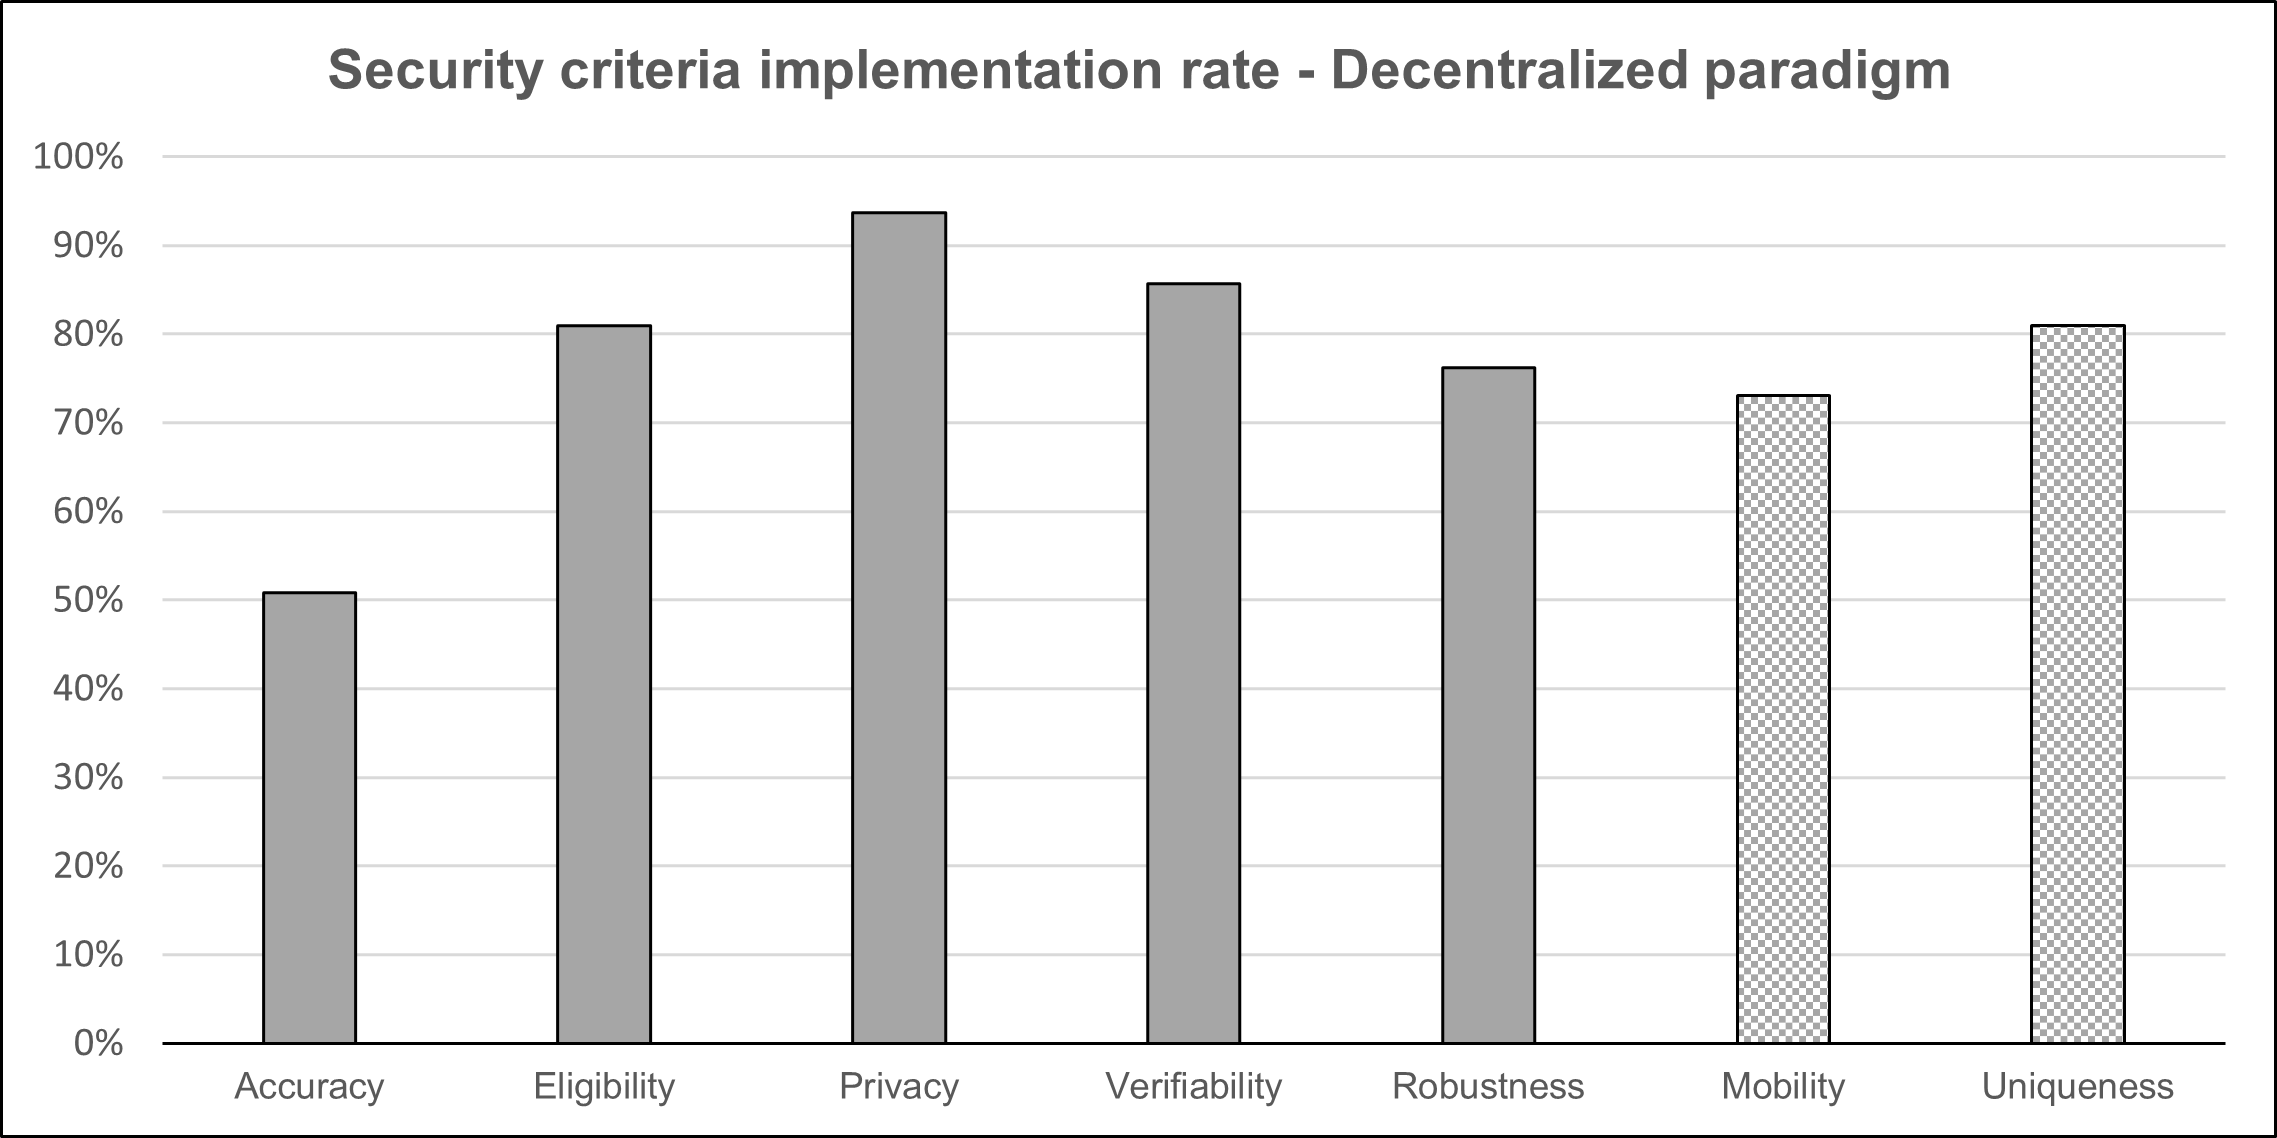
\includegraphics[width=\columnwidth]{Images/almei5.png}
    \caption{Statistical analysis of implementation rate.}
    \label{fig:implementation-rate-decentralized}
\end{figure}

The use of a blockchain in an e-voting solution promptly nullifies the usefulness of cryptographic methods such as a \textit{public bulletin board} and \textit{anonymous communication channel}. The blockchain's transparency regarding data access makes these methods redundant in a decentralised context. As such, we removed these methods from consideration in the decentralised analysis. Also, proposals that did not use or specify any of the cryptographic methods considered are omitted, which reduced the initial set considered from \textit{63} to \textit{34} publications.

\paragraph{Systematic Map}
The results from the application of the classification strategy indicated are compiled in Table \ref{tbl:table5}, also organised in chronological order.

\begin{table*}[htbp]
    \caption{Cryptographic methods identified in decentralized literature.}
    \begin{adjustwidth}{-2cm}{}
        \begin{tabular}{m{4.4cm} c >{\centering\arraybackslash}m{1.7cm} c >{\centering\arraybackslash}m{6cm} >{\centering\arraybackslash} m{1.0cm} >{\centering\arraybackslash}m{14.9cm}} % Column alignments
            \toprule
            \multirow{3.5}{=}{\textbf{\footnotesize{References}}}          & \multicolumn{4}{c}{\textbf{Cryptographic Protocols}}                                                                                                                                                             \\
            \cline{2-5}
            \vspace{0.5cm}
            \multirow{2}{=}{}                                              & \parbox[m]{1.7cm}{\footnotesize{Homomorphism}}       & \footnotesize{Blind/Ring Signatures} & \footnotesize{Mix-Nets} & \footnotesize{Cryptographic Proof}                                                       \\
            \hline
            \footnotesize{Zhao et al. (2016) \cite{Zhao2016}}              & {}                                                   & {}                                   & {}                      & \footnotesize{zk-SNARKS (Zero-Knowledge Succinct Non-Interactive Argument of Knowledge)} \\
            \hline
            \footnotesize{Cruz and Kaji (2016) \cite{Cruz2016}}            & {}                                                   & $ \checkmark $                       & {}                      & {}                                                                                       \\
            \hline
            \footnotesize{McCorry (2017) \cite{McCorry2017}}               & {}                                                   & {}                                   & {}                      & \footnotesize{Schnorr and On-out-of-two Zero Knowledge Proofs}                           \\
            \hline
            \footnotesize{Shaheen (2017) \cite{Shaheen2017}}               & $ \checkmark $                                       & $ \checkmark $                       & {}                      & {}                                                                                       \\
            \hline
            \footnotesize{Liu and Wang (2017) \cite{Liu2017}}              & {}                                                   & $ \checkmark $                       & {}                      & {}                                                                                       \\
            \hline
            \footnotesize{Hardwick et al. (2018) \cite{Hardwick2018}}      & {}                                                   & $ \checkmark $                       & {}                      & {}                                                                                       \\
            \hline
            \footnotesize{Wang et al. (2018) \cite{Wang2018}}              & $ \checkmark $                                       & $ \checkmark $                       & {}                      & \footnotesize{Groth-Sahai Non-Interactive Zero-Knowledge Proof}                          \\
            \hline
            \footnotesize{Hsiao (2018) \cite{Hsiao2018}}                   & $ \checkmark $                                       & {}                                   & {}                      & {}                                                                                       \\
            \hline
            \footnotesize{Chaieb et al. (2018) \cite{Chaieb2018}}          & $ \checkmark $                                       & {}                                   & {}                      & {}                                                                                       \\
            \hline
            \footnotesize{Zhang et al. (2018) \cite{Zhang2018}}            & $ \checkmark $                                       & {}                                   & {}                      & {}                                                                                       \\
            \hline
            \footnotesize{Dagher et al. (2018) \cite{Dagher2018}}          & $ \checkmark $                                       & {}                                   & {}                      & {}                                                                                       \\
            \hline
            \footnotesize{Bartolucci et al. (2018) \cite{Bartolucci2018}}  & {}                                                   & {}                                   & $ \checkmark $          & {}                                                                                       \\
            \hline
            \footnotesize{Perez and Ceesay (2018) \cite{Perez2018}}        & $ \checkmark $                                       & {}                                   & {}                      & {}                                                                                       \\
            \hline
            \footnotesize{Yu et al. (2018) \cite{Yu2018}}                  & {}                                                   & $ \checkmark $                       & {}                      & \footnotesize{Non-specified Zero-Knowledge Proofs}                                       \\
            \hline
            \footnotesize{Matile et al. (2019) \cite{Matile2019}}          & $ \checkmark $                                       & {}                                   & {}                      & {}                                                                                       \\
            \hline
            \footnotesize{Murtaza et al. (2019) \cite{Murtaza2019}}        & {}                                                   & {}                                   & {}                      & \footnotesize{zk-SNARKS}                                                                 \\
            \hline
            \footnotesize{Lyu et al. (2019) \cite{Lyu2019}}                & {}                                                   & $ \checkmark $                       & {}                      & {}                                                                                       \\
            \hline
            \footnotesize{Chaieb et al. (2019) \cite{Chaieb2019}}          & $ \checkmark $                                       & $ \checkmark $                       & {}                      & {}                                                                                       \\
            \hline
            \footnotesize{Lopes et al. (2019) \cite{Lopes2019}}            & $ \checkmark $                                       & {}                                   & {}                      & {}                                                                                       \\
            \hline
            \footnotesize{Zhang et al. (2019) \cite{Zhang2019a}}           & $ \checkmark $                                       & $ \checkmark $                       & {}                      & \footnotesize{Non-Interactive Zero-Knowledge Proof}                                      \\
            \hline
            \footnotesize{Mols and Vasilomanolakis (2020) \cite{Mols2020}} & {}                                                   & {}                                   & {}                      & \footnotesize{zk-SNARKS}                                                                 \\
            \hline
            \footnotesize{Yang et al. (2020) \cite{Yang2020}}              & $ \checkmark $                                       & $ \checkmark $                       & {}                      & \footnotesize{Non-specified Zero-Knowledge Proof}                                        \\
            \hline
            \footnotesize{Chaieb et al. (2020) \cite{Chaieb2020}}          & {}                                                   & {}                                   & $ \checkmark $          & \footnotesize{Non-Interactive Zero-Knowledge Proof}                                      \\
            \hline
            \footnotesize{Killer et al. (2020) \cite{Killer2020}}          & $ \checkmark $                                       & {}                                   & {}                      & {}                                                                                       \\
            \hline
            \footnotesize{Shao et al. (2020) \cite{Shao2020}}              & {}                                                   & $ \checkmark $                       & {}                      & \footnotesize{Non-Interactive Zero-Knowledge Proof}                                      \\
            \hline
            \footnotesize{Xu and Cao (2020) \cite{Xu2020}}                 & {}                                                   & {}                                   & {}                      & \footnotesize{Non-specified Zero-Knowledge Proof}                                        \\
            \hline
            \footnotesize{Zhang et al. (2020) \cite{Zhang2020}}            & $ \checkmark $                                       & $ \checkmark $                       & {}                      & {}                                                                                       \\
            \hline
            \footnotesize{Dimitriou (2022) \cite{Dimitriou2020}}           & {}                                                   & {}                                   & {}                      & \footnotesize{zk-SNARKS and Pedersen commitments}                                        \\
            \hline
            \footnotesize{Han et al. (2020) \cite{Han2020}}                & {}                                                   & {}                                   & {}                      & \footnotesize{Non-specified Zero-Knowledge Proof}                                        \\
            \hline
            \footnotesize{Zhou et al. (2020) \cite{Zhou2020}}              & {}                                                   & $ \checkmark $                       & {}                      & {}                                                                                       \\
            \hline
            \footnotesize{Takabatake et al. (2021) \cite{Takabatake2021}}  & {}                                                   & {}                                   & {}                      & \footnotesize{Zerocoin's Zero Knowledge Proof system}                                    \\
            \hline
            \footnotesize{Li et al. (2021) \cite{Li2021}}                  & $ \checkmark $                                       & {}                                   & {}                      & \footnotesize{Non-Interactive Zero-Knowledge Proof}                                      \\
            \hline
            \footnotesize{Hu et al. (2022) \cite{Hu2022}}                  & {}                                                   & $ \checkmark $                       & {}                      & {}                                                                                       \\
            \hline
            \footnotesize{Li et al. (2020) \cite{Li2022}}                  & {}                                                   & {}                                   & {}                      & \footnotesize{Non-specified Zero-Knowledge Proof}                                        \\
            \bottomrule
        \end{tabular}
    \end{adjustwidth}
    \label{tbl:table5}
\end{table*}

\paragraph{Analysis of Results}
Decentralised proposals use homomorphic properties of cryptosystems at a slightly higher rate than their centralised counterparts, namely 45.5\% against 34\%, explainable by the public nature of most of the blockchain implementations considered. In a typical system, vote data is encrypted as soon as possible, ideally after the voter has made the choice. It then remains encrypted for as long as the process does not depend on any of the encrypted data. But whenever any counting needs to happen, either partial calculations or the final tally, vote data needs to be decrypted to perform these types of arithmetic operations, unless a homomorphic cryptosystem is used instead. In this scenario, using a threshold cryptosystem with homomorphic characteristics is an advantage since it allows executing operations in the ciphertext domain, which reduces the decrypting operations to the final tally only. This concept was present in the centralised proposals, but it is more evident when a blockchain, particularly a public one, is used. Regarding the cryptosystems used for this purpose, from the authors that did specify them, the majority are divided between the ElGamal cryptosystem \cite{ElGamal1984}, as in the case of \cite{Matile2019}, \cite{Wang2018}, \cite{Chaieb2018}, \cite{Yang2020}, \cite{Killer2020} and \cite{Li2021}, and the Paillier cryptosystem \cite{OKeeffe2008}, as it is the case for \cite{Hsiao2018}, \cite{Zhang2018}, \cite{Dagher2018}, \cite{Chaieb2019}, \cite{Lopes2019}, \cite{Zhang2019a} and \cite{Zhang2020}.
\par
The usage of \textit{blind/ring signatures} also registers an increase from 31\% to 45.5\% in decentralised literature for the same reasons. Blind or ring-signed ballots are a good method to privatise voter data in a public channel, like a blockchain, and this is verifiable in the analysed literature.
\par
Both \textit{blind/ring signatures} and \textit{homomorphism} can be used to protect data in a publicly accessible channel, but the process in which this happens and the properties of the hidden data are different, which means that some proposals can use both without incurring redundancy: \textit{Blind/Ring signatures} are used to protect voter data written into a blockchain, whereas \textit{homomorphism} is used so that tallies can be computed without decrypting partial results. Proposals such as \cite{Shaheen2017}, \cite{Wang2018}, \cite{Chaieb2019}, \cite{Zhang2019a}, \cite{Yang2020} and \cite{Zhang2020} implement both of these tools in their solutions.
\par
The most evident contrast between paradigms shows itself in the implementation of \textit{Mix-Nets}. Blockchains are not necessarily technologically comparable to these, but they achieve similar results nonetheless due to their anonymity features, which is the main objective when employing \textit{Mix-Nets} in past proposals. Only two of the works surveyed implement structures that, though not exactly the \textit{Mix-Net} concept defined in Section \ref{centralized_mix_nets}, are similar enough to be mentioned in this analysis. \cite{Bartolucci2018} uses a technique called \textit{Circle Shuffle} which resembles a \textit{Mix-Net} and, similarly to it, is used to de-link voter data from their votes, i.e., to implement \textit{Privacy}. \cite{Chaieb2020} employs a "new mix network protocol", which they claim to be used to implement coercion resistance in their solution but do not present any additional details about its implementation.
\par
Finally, as it has been the trend so far, decentralised proposals also have a higher rate of cryptographic proof usage, and it can be attributed to the same reasons considered so far. Due to blockchain's public nature, which conflicts with the necessity of maintaining voter privacy in these systems, cryptographic proofs, with an emphasis on zero-knowledge ones, are often used to achieve verifiability while maintaining voter privacy in a public information system. Some authors are more specific than others regarding the actual type of proof used, as can be seen in Table \ref{tbl:table5}, but ultimately their goal is the same.

\paragraph{Characteristic Elements of Decentralised e-Voting Proposals}
\par
\textbf{Blockchain scope}
\par
\label{blockchain-type-access-control}
Regarding their scope, blockchains can fall into one of three categories:
\begin{enumerate}
    \item {Public blockchains use encryption and sequences of cryptographic hashes to enact data privacy. Bitcoin and Ethereum are good examples of public blockchains. These blockchains provide better information transparency and auditability, but a cost in performance and through the imposition of a cost model, namely the requirement of a small quantity of cryptocurrency to be paid (gas) to operate with this type of blockchain, from cryptocurrency transactions to smart contract executions, as a protection strategy against malicious actors and unoptimized code \cite{Xu2017}}.

    \item {Private blockchains are opposed to the last ones, being only open to members of a particular organisation or group. External access for reading and transaction execution is forbidden. Likewise, participation as a network node is limited to members of the group or organisation. Due to these access restrictions, these blockchains do present a level of centralization in their implementation through the presence of a central authority that manages participation in the organisation and therefore in the network. A smaller network means higher block rates and transaction speeds due to less restrictive consensus protocols, as well as less communication required to achieve consensus, which also makes these networks more scalable \cite{Viriyasitavat2019}.}

    \item {Consortium blockchains sit somewhere between the two other types discussed thus far, a hybrid between private and public. These are suitable for semi-closed groups of organisations or a consortium, where the name derives from. Access to these blockchains is conditioned, just like in private chains, but the degree of data openness and access regulation varies depending on the rules agreed upon within the consortium. The nodes that compose the blockchain network are pre-selected internally, but the network can have nodes added to it if these get properly authorized. Their performance regarding block rates, transaction speeds, and scalability is also between the public and private specs \cite{Xinyi2018}}.
\end{enumerate}

\par
\textbf{Blockchain Permissions}
\par
Data in a blockchain can be restricted for \emph{read} and \emph{write} operations, and the permissions associated to these operations are also an important defining element for a blockchain. As defined in Section \ref{mining-consensus}, new data can only be appended to a blockchain by mining a new block into it. This means that a blockchain that restricts \emph{write} operations is actually preventing nodes from participating in the mining process.
\par
A blockchain that regulates which nodes have \emph{read} permissions is denoted as a \textit{permissioned} blockchain. Otherwise, it is considered a \textit{permissionless} blockchain. Regarding the \emph{write} operation, a blockchain can be of one of the two types indicated as well, but given that there are no examples of blockchains that regulate \emph{reads} but not \emph{writes}, i.e., a blockchain that only allows select actors to read its data but at the same time anyone is free to join it as a mining node, from these designations, three possible scenarios follow for each blockchain:
\begin{itemize}
    \item{Permissionless reads and writes: This is the case for most public blockchains, of which Bitcoin and Ethereum are good examples. Anyone is free to read the block contents, and, theoretically, anyone can participate as a node and mine new blocks. Realistically, for PoW blockchains, the popularity of the blockchain, along with the price of the associated cryptocurrency, may create a steep entry price in terms of hardware investment to be able to actively compete with existing nodes. PoS blockchains are not as hardware-dependent as PoW ones, but the minimum stake required to be considered by the algorithm that selects the new block creator may also be outside the budget of most people. But these are economic barriers to entry. From a protocol standpoint, there are no permission-based rules preventing anonymous nodes from joining and participating in the consensus of the network.}

    \item{Permissionless reads but permissioned writes: Anyone is free to read the contents of this blockchain, but the consensus protocol is restricted to pre-selected nodes. Ripple is a good example of a public blockchain that implements this permission set: only nodes belonging to a \textit{unique node list} are able to validate transactions and produce new blocks, while users are able to consult the data in it.}

    \item{Permissioned reads and writes: All access is conditioned in these types of blockchains. A machine needs to be granted access before it can even access the structure for reading purposes, typically from a central authority of some type.}
\end{itemize}

Access is independent of the scope, but only to a point. Anyone creating a blockchain is free to create it under the scope and access permissions desired. Even though it is not practical, one can create a public blockchain with permissioned access to both reads and writes. Or a private blockchain without any read or write permissions. From a functional standpoint, these extreme cases do not make much sense, but they are still technically viable. Realistically, most public blockchains tend to be free for read and write purposes, whereas most private ones tend to regulate these operations, but this is not a strict rule.
\par
Due to this fluidity, we opted to focus solely on the scope of the blockchain used in the proposed solution and omit its permission set since it is often not indicated in the publications.

\par
\textbf{Blockchain Types}
\par
Our analysis characterises in which one of these groups the blockchain used in each proposal falls, as well as the specific type or brand of blockchain used if indicated. Sometimes the indication of the type is enough to infer about the access control. For example, if a proposal specifies the usage of Bitcoin's blockchain, we can infer the usage of a public blockchain, given that Bitcoin does not offer any other type.
\par
The characterization of the type of blockchain used is typically straightforward, except for the Ethereum network. Being the first network to offer explicit smart contract support and being a constant target of improvements unlike other, more static networks like Bitcoin, if a solution uses this network, it is important to specify which version or specific type was actually used, namely, if it was based on the initial, PoW-based version, Ethereum 1.0, or the newer, PoS-based Ethereum 2.0, which has appeared in later proposals. Besides these, Ethereum also provides custom implementations based on the Go programming language that can be used to implement private or consortium networks, as well as variants that use other consensus algorithms, such as the Ropsten test network, for example. This one is an Ethereum network, but it adopts Proof-of-Authority as a consensus algorithm. For the sake of simplicity, a more granular approach where only the major versions of Ethereum and any custom blockchains based on this protocol (Go-Ethereum being the most popular) are used as classes.
\par
Some proposals do explore a blockchain-based solution from a more generalist perspective, focusing on the desired mechanics rather than the implementation details. As such, these do not specify a blockchain type, the assumption being that the solution is general enough to be implemented in most blockchain solutions available. In these cases, we indicate this option as using a \textit{generic} blockchain type.
\par
More recent proposals take this step further in this regard, and instead of opting for an existing solution or even assuming a generalised blockchain, they indicate the use of a proprietary blockchain, i.e., a blockchain built from scratch and tailored to the application needs. This is a consequence of the popularisation and generalisation of blockchain as a concept. With a well-defined set of basic functionalities and plenty of practical examples to use as guidance, some researchers were able to develop custom blockchains. These cases were identified using a \textit{proprietary} blockchain type.

\par
\textbf{Levels of Decentralization}
\par
Some proposals analysed seem to be constructed just as proof that it is indeed possible to establish a fully decentralised e-voting system using blockchain alone. These proposals put themselves on the decentralised extreme of the spectrum, whereas all the publications reviewed in Section \ref{centralized-analysis} are on the opposite side.
\par
These extreme proposals are minimal. Most publications propose a hybrid system that sits somewhere between these two extremes. Therefore, it is useful to characterise where the proposals sit in this regard, namely to infer about the advantages, disadvantages, and problems of placing the system at different points of the spectrum.
\par
Examples of typical centralising elements that we look for include centralised databases (the most popular) and trusted third parties, such as election organisers and/or governmental agencies.
\par
\textbf{Blockchain Voting Methods}
\par
The approach taken to implement the votes themselves originated from a variety of ingenious ways to use the features offered by blockchains. This derives directly from the fact that, so far, no blockchain has been created for the sole purpose of providing support for e-voting exercises, unlike the proposals analysed in Section \ref{centralized-analysis}. The most rigid ones were created primarily as digital currency ledgers, whereas more flexible ones are similar to general-purpose computers, i.e., need extra configuration to be able to support an e-voting system. Researchers were forced to use creative methods to be able to use blockchains for that purpose. Analysing how these methods evolved is an important aspect to include in this study.
\par
This classification exercise infers the popularity of the methods identified. During our analysis, we encountered a variety of techniques used in the publications. These were grouped into the following sets:
\begin{enumerate}
    \item{Cryptocurrency/Token Transactions:}
          Using transactional metadata to transport non-financial information on a cryptocurrency-based blockchain is a popular approach due to its simplicity. Most blockchains provide meta fields that can be used to write information that may not be related to the transactional action. A perfect example of this is the \textbf{OP\_RETURN} meta field available in Bitcoin's transaction format.

    \item{New Blockchain Block:}
          Another approach is to represent a vote as a new block added to a blockchain, representing a specific voting option. This allows for quick tally computations since the size of a chain is a basic statistic in these constructs. But the feasibility of this option is minimal, especially if the target is a public blockchain, where appending new blocks is regulated by restrictive consensus protocols. But it may be a suitable option for a private blockchain with its own rules to add new blocks that do not impose a block rate as public chains do.

    \item{Smart Contract/Chaincode Execution:}
          Using smart contracts to establish independent and open code that can be automatically executed to increase a count is a verifiable trend in this context. Publications based on early blockchains that did not provide this support displayed imaginative ways to use a financial tool for democratic purposes. But once smart contracts became more popular and understood, this feature was present in relevant research almost immediately. Smart contracts enable a level of transparency and human freedom that, along with the deterministic nature of their operation, increase the security of the system.
          \par
          A significant number of authors created custom blockchains to deploy their solutions, with Hyperledger Fabric among the more popular options. Hyperledger can also run scripts, which are referred to as chaincodes in that context, in a decentralised fashion, which are similar to smart contracts.
          \par
          Smart contracts are the best option considered so far for this specific purpose. Not only do they allow for the establishment of specific rules for the voting process, but they also allow for the maintenance of system-wide variables.
\end{enumerate}


\paragraph{Systematic Map}
Applying the mapping process and framing the analysis within the research questions defined in section \ref{specific-research-questions} produced tables \ref{tbl:table6} and \ref{tbl:table7}.

\begin{table*}[htbp]
    \caption{Characterization of decentralized e-voting system in the literature.}
    \begin{adjustwidth}{-2cm}{}
        \begin{tabular}{m{4.4cm} >{\centering\arraybackslash}m{2.9cm} >{\centering\arraybackslash}m{1.0cm} >{\centering\arraybackslash}m{1.0cm} >{\centering\arraybackslash}m{1.5cm} >{\centering\arraybackslash}m{3.6cm}} % Column alignments
            \toprule
            \multirow{2.5}{=}{\textbf{References}}                              & \multicolumn{2}{c}{Blockchain characteristics} & \multirow{2.5}{=}{\footnotesize{Smart Contract}} & \multirow{2.5}{=}{\footnotesize{Centralizing Element}} & \multirow{2.5}{*}{\footnotesize{Vote Implementation}}                                              \\
            \cline{2-3}
            \vspace{0.25cm}
            \multirow{2}{=}{}                                                   & \footnotesize{Type}                            & \footnotesize{Access}                            & \multirow{2}{=}{}                                      & \multirow{2}{=}{}                                     & \multirow{2}{=}{}                          \\
            \hline
            \footnotesize{Barnes (2016) \cite{Barnes2016}}                      & \footnotesize{Proprietary}                     & \footnotesize{Public}                            & {}                                                     & {}                                                    & \footnotesize{Token transaction}           \\
            \hline
            \footnotesize{Kirby (2016) \cite{Kirby2016}}                        & \footnotesize{Proprietary}                     & \footnotesize{Private}                           & {}                                                     & $ \checkmark $                                        & \footnotesize{Cryptocurrency transactions} \\
            \hline
            \footnotesize{Zhao and Chan (2016) \cite{Zhao2016}}                 & \footnotesize{Bitcoin}                         & \footnotesize{Public}                            & {}                                                     & {}                                                    & \footnotesize{Cryptocurrency transactions} \\
            \hline
            \footnotesize{Cruz and Kaji (2016) \cite{Cruz2016}}                 & \footnotesize{Bitcoin}                         & \footnotesize{Public}                            & {}                                                     & $ \checkmark $                                        & \footnotesize{Cryptocurrency transactions} \\
            \hline
            \footnotesize{Ben Ayed (2017) \cite{BenAyed2017}}                   & \footnotesize{Proprietary}                     & \footnotesize{Private}                           & {}                                                     & {}                                                    & \footnotesize{New blockchain block}        \\
            \hline
            \footnotesize{McCorry (2017) \cite{McCorry2017}}                    & \footnotesize{Ethereum 1.0 (PoW)}              & \footnotesize{Public}                            & $ \checkmark $                                         & $ \checkmark $                                        & \footnotesize{Smart Contract execution}    \\
            \hline
            \footnotesize{Bistarelli (2017) \cite{Bistarelli2017}}              & \footnotesize{Bitcoin}                         & \footnotesize{Public}                            & {}                                                     & $ \checkmark $                                        & \footnotesize{Cryptocurrency transactions} \\
            \hline
            \footnotesize{Lee (2017) \cite{Lee2017}}                            & \footnotesize{Bitcoin}                         & \footnotesize{Public}                            & {}                                                     & $ \checkmark $                                        & \footnotesize{Cryptocurrency transactions} \\
            \hline
            \footnotesize{Shaheen (2017) \cite{Shaheen2017}}                    & \footnotesize{Bitcoin}                         & \footnotesize{Public}                            & {}                                                     & {}                                                    & \footnotesize{Token transaction}           \\
            \hline
            \footnotesize{Wu (2017) \cite{Wu2017}}                              & \footnotesize{Bitcoin}                         & \footnotesize{Public}                            & {}                                                     & $ \checkmark $                                        & \footnotesize{Cryptocurrency transactions} \\
            \hline
            \footnotesize{Liu and Wang (2017) \cite{Liu2017}}                   & \footnotesize{Generic}                         & {}                                               & {}                                                     & $ \checkmark $                                        & \footnotesize{Cryptocurrency transactions} \\
            \hline
            \footnotesize{Hardwick et al. (2018) \cite{Hardwick2018}}           & \footnotesize{Ethereum 1.0 (PoW)}              & \footnotesize{Private}                           & {}                                                     & $ \checkmark $                                        & \footnotesize{Cryptocurrency transactions} \\
            \hline
            \footnotesize{Wang et al. (2018) \cite{Wang2018}}                   & \footnotesize{Ethereum 1.0 (PoW)}              & \footnotesize{Public}                            & $ \checkmark $                                         & $ \checkmark $                                        & \footnotesize{Smart Contract execution}    \\
            \hline
            \footnotesize{Ko\c{c} (2018) \cite{Koc2018}}                        & \footnotesize{Ethereum 1.0 (PoW)}              & \footnotesize{Public}                            & $ \checkmark $                                         & $ \checkmark $                                        & \footnotesize{Smart Contract execution}    \\
            \hline
            \footnotesize{Hsiao (2018) \cite{Hsiao2018}}                        & \footnotesize{Ethereum 1.0 (PoW)}              & \footnotesize{Public}                            & $ \checkmark $                                         & $ \checkmark $                                        & \footnotesize{Smart Contract execution}    \\
            \hline
            \footnotesize{Chaieb et al. (2018) \cite{Chaieb2018}}               & \footnotesize{Ethereum 1.0 (PoW)}              & \footnotesize{Public}                            & $ \checkmark $                                         & $ \checkmark $                                        & \footnotesize{Smart Contract execution}    \\
            \hline
            \footnotesize{Khan et al. (2018) \cite{Khan2018}}                   & \footnotesize{Multichain}                      & \footnotesize{Public}                            & {}                                                     & $ \checkmark $                                        & \footnotesize{New blockchain block}        \\
            \hline
            \footnotesize{Zhang et al. (2018) \cite{Zhang2018}}                 & \footnotesize{Hyperledger Fabric}              & \footnotesize{Private}                           & $ \checkmark $                                         & {}                                                    & \footnotesize{Token transaction}           \\
            \hline
            \footnotesize{Lai et al. (2018) \cite{Lai2018}}                     & \footnotesize{Ethereum 1.0 (PoW)}              & \footnotesize{Public}                            & $ \checkmark $                                         & $ \checkmark $                                        & \footnotesize{Cryptocurrency transactions} \\
            \hline
            \footnotesize{Dagher et al. (2018) \cite{Dagher2018}}               & \footnotesize{Go-Ethereum}                     & \footnotesize{Private}                           & $ \checkmark $                                         & $ \checkmark $                                        & \footnotesize{Smart Contract execution}    \\
            \hline
            \footnotesize{Bartolucci et al. (2018) \cite{Bartolucci2018}}       & \footnotesize{Bitcoin}                         & \footnotesize{Public}                            & {}                                                     & $ \checkmark $                                        & \footnotesize{Cryptocurrency transactions} \\
            \hline
            \footnotesize{Hj\'{a}lmarsson et al. (2018) \cite{Hjalmarsson2018}} & \footnotesize{Go-Ethereum}                     & \footnotesize{Private}                           & $ \checkmark $                                         & $ \checkmark $                                        & \footnotesize{Smart Contract execution}    \\
            \hline
            \footnotesize{Shukla et al. (2018) \cite{Shukla2018}}               & \footnotesize{Ethereum 1.0 (PoW)}              & \footnotesize{Public}                            & $ \checkmark $                                         & $ \checkmark $                                        & \footnotesize{Smart Contract execution}    \\
            \hline
            \footnotesize{Khoury et al. (2018) \cite{Khoury2018}}               & \footnotesize{Ethereum 1.0 (PoW)}              & \footnotesize{Public}                            & $ \checkmark $                                         & $ \checkmark $                                        & \footnotesize{Smart Contract execution}    \\
            \hline
            \footnotesize{Perez and Ceesay (2018) \cite{Perez2018}}             & \footnotesize{Ethereum 1.0 (PoW)}              & \footnotesize{Public}                            & $ \checkmark $                                         & {}                                                    & \footnotesize{Smart Contract execution}    \\
            \hline
            \footnotesize{Yu et al. (Yu2018) \cite{Yu2018}}                     & \footnotesize{Hyperledger Fabric}              & \footnotesize{Private}                           & $ \checkmark $                                         & $ \checkmark $                                        & \footnotesize{Chaincode execution}         \\
            \hline
            \footnotesize{Matile et al. (2019) \cite{Matile2019}}               & \footnotesize{Proprietary}                     & \footnotesize{Private}                           & {}                                                     & $ \checkmark $                                        & \footnotesize{Token transaction}           \\
            \hline
            \footnotesize{Vo-Cao-Thuy et al. (2019) \cite{Vo-Cao-Thuy2019}}     & \footnotesize{Ethereum 1.0 (PoW)}              & \footnotesize{Public}                            & $ \checkmark $                                         & $ \checkmark $                                        & \footnotesize{Token transaction}           \\
            \hline
            \footnotesize{Bosri et al. (2019) \cite{Bosri2019}}                 & \footnotesize{Ethereum 1.0 (PoW)}              & \footnotesize{Public}                            & {}                                                     & $ \checkmark $                                        & \footnotesize{Token transaction}           \\
            \hline
            \footnotesize{Yi (2019) \cite{Yi2019}}                              & \footnotesize{Bitcoin/Zerocoin}                & \footnotesize{Public}                            & {}                                                     & $ \checkmark $                                        & \footnotesize{Cryptocurrency transactions} \\
            \hline
            \footnotesize{Singh and Chatterjee (2019) \cite{Singh2019}}         & \footnotesize{Generic}                         & \footnotesize{Private}                           & {}                                                     & $ \checkmark $                                        & \footnotesize{New blockchain block}        \\
            \bottomrule
        \end{tabular}
    \end{adjustwidth}
    \label{tbl:table6}
\end{table*}

\begin{table*}[htbp]
    \caption{Characterization of decentralized e-voting system in literature.}
    \begin{adjustwidth}{-1cm}{}
        \begin{tabular}{m{4.4cm} >{\centering\arraybackslash}m{2.9cm} >{\centering\arraybackslash}m{1.0cm} >{\centering\arraybackslash}m{1.0cm} >{\centering\arraybackslash}m{1.5cm} >{\centering\arraybackslash}m{3.6cm}} % Column alignments
            \toprule
            \multirow{2.5}{=}{\textbf{References}}                         & \multicolumn{2}{c}{Blockchain characteristics} & \multirow{2.5}{=}{\footnotesize{Smart Contract}} & \multirow{2.5}{=}{\footnotesize{Centralizing Element}} & \multirow{2.5}{*}{\footnotesize{Vote Implementation}}                                              \\
            \cline{2-3}
            \vspace{0.25cm}
            \multirow{2}{=}{}                                              & \footnotesize{Type}                            & \footnotesize{Access}                            & \multirow{2}{=}{}                                      & \multirow{2}{=}{}                                     & \multirow{2}{=}{}                          \\
            \hline
            \footnotesize{Adiputra et al. (2019) \cite{Adiputra2019}}      & \footnotesize{Generic}                         & \footnotesize{Private}                           & {}                                                     & $ \checkmark $                                        & \footnotesize{New blockchain block}        \\
            \hline
            \footnotesize{Murtaza et al. (2019) \cite{Murtaza2019}}        & \footnotesize{Proprietary}                     & \footnotesize{Private}                           & {}                                                     & $ \checkmark $                                        & \footnotesize{Token transaction}           \\
            \hline
            \footnotesize{Lyu et al. (2019) \cite{Lyu2019}}                & \footnotesize{Go-Ethereum}                     & \footnotesize{Private}                           & $ \checkmark $                                         & $ \checkmark $                                        & \footnotesize{Smart Contract execution}    \\
            \hline
            \footnotesize{Seftyanto et al. (2019) \cite{Seftyanto2019}}    & \footnotesize{Hyperledger Fabric}              & \footnotesize{Private}                           & $ \checkmark $                                         & $ \checkmark $                                        & \footnotesize{Token transaction}           \\
            \hline
            \footnotesize{Chaieb et al. (2019) \cite{Chaieb2019}}          & \footnotesize{Generic}                         & \footnotesize{Private}                           & $ \checkmark $                                         & $ \checkmark $                                        & \footnotesize{New blockchain block}        \\
            \hline
            \footnotesize{Faour (2019) \cite{Faour2019}}                   & \footnotesize{Proprietary}                     & \footnotesize{Public}                            & $ \checkmark $                                         & {}                                                    & \footnotesize{Smart Contract execution}    \\
            \hline
            \footnotesize{Lopes et al. (2019) \cite{Lopes2019}}            & \footnotesize{Ethereum 1.0 (PoW)}              & \footnotesize{Public}                            & $ \checkmark $                                         & $ \checkmark $                                        & \footnotesize{Smart Contract execution}    \\
            \hline
            \footnotesize{Zhang et al. (2019) \cite{Zhang2019a}}           & \footnotesize{Ethereum 1.0 (PoW)}              & \footnotesize{Public}                            & $ \checkmark $                                         & $ \checkmark $                                        & \footnotesize{Smart Contract execution}    \\
            \hline
            \footnotesize{Mols and Vasilomanolakis (2020) \cite{Mols2020}} & \footnotesize{Ethereum 1.0 (PoW)}              & \footnotesize{Public}                            & $ \checkmark $                                         & $ \checkmark $                                        & \footnotesize{Smart Contract execution}    \\
            \hline
            \footnotesize{Yang et al. (2020) \cite{Yang2020}}              & \footnotesize{Generic}                         & \footnotesize{Private}                           & $ \checkmark $                                         & {}                                                    & \footnotesize{Token transaction}           \\
            \hline
            \footnotesize{Chaieb and Yousfi (2020) \cite{Chaieb2020}}      & \footnotesize{Monero}                          & \footnotesize{Public}                            & {}                                                     & $ \checkmark $                                        & \footnotesize{Cryptocurrency transactions} \\
            \hline
            \footnotesize{Sadia et al. (2020) \cite{Sadia2020}}            & \footnotesize{Generic}                         & \footnotesize{Private}                           & $ \checkmark $                                         & {}                                                    & \footnotesize{Token transaction}           \\
            \hline
            \footnotesize{Killer et al. (2020) \cite{Killer2020}}          & \footnotesize{Proprietary}                     & \footnotesize{Consortium}                        & $ \checkmark $                                         & $ \checkmark $                                        & \footnotesize{Smart Contract execution}    \\
            \hline
            \footnotesize{Shao et al. (2020) \cite{Shao2020}}              & \footnotesize{Go-Ethereum}                     & \footnotesize{Private}                           & $ \checkmark $                                         & $ \checkmark $                                        & \footnotesize{Smart Contract execution}    \\
            \hline
            \footnotesize{Xu and Cao (2020) \cite{Xu2020}}                 & \footnotesize{Go-Ethereum}                     & \footnotesize{Private}                           & $ \checkmark $                                         & $ \checkmark $                                        & \footnotesize{Smart Contract execution}    \\
            \hline
            \footnotesize{Zaghloul et al. (2020) \cite{Zaghloul2020}}      & \footnotesize{Generic}                         & \footnotesize{Public}                            & $ \checkmark $                                         & $ \checkmark $                                        & \footnotesize{Smart Contract execution}    \\
            \hline
            \footnotesize{Zhang et al. (2020) \cite{Zhang2020}}            & \footnotesize{Generic}                         & \footnotesize{Private}                           & $ \checkmark $                                         & $ \checkmark $                                        & \footnotesize{Smart Contract execution}    \\
            \hline
            \footnotesize{Dimitriou (2020) \cite{Dimitriou2020}}           & \footnotesize{Bitcoin}                         & \footnotesize{Public}                            & {}                                                     & $ \checkmark $                                        & \footnotesize{Cryptocurrency transactions} \\
            \hline
            \footnotesize{Alvi et al. (2020) \cite{Alvi2020}}              & \footnotesize{Ethereum 2.0 (PoS)}              & \footnotesize{Public}                            & $ \checkmark $                                         & $ \checkmark $                                        & \footnotesize{Smart Contract execution}    \\
            \hline
            \footnotesize{Han et al. (2020) \cite{Han2020}}                & \footnotesize{Proprietary}                     & \footnotesize{Consortium}                        & {}                                                     & {}                                                    & \footnotesize{Token transaction}           \\
            \hline
            \footnotesize{Zhou et al. (2020) \cite{Zhou2020}}              & \footnotesize{Hyperledger Fabric}              & \footnotesize{Private}                           & $ \checkmark $                                         & {}                                                    & \footnotesize{Chaincode execution}         \\
            \hline
            \footnotesize{Vivek et al. (2020) \cite{Vivek2020}}            & \footnotesize{Hyperledger Sawtooth}            & \footnotesize{Private}                           & $ \checkmark $                                         & $ \checkmark $                                        & \footnotesize{Chaincode execution}         \\
            \hline
            \footnotesize{Takabatake et al. (2021) \cite{Takabatake2021}}  & \footnotesize{Zerocoin}                        & \footnotesize{Public}                            & $ \checkmark $                                         & $ \checkmark $                                        & \footnotesize{Cryptocurrency transactions} \\
            \hline
            \footnotesize{Larriba et al. (2021) \cite{Larriba2021}}        & \footnotesize{Monero}                          & \footnotesize{Public}                            & {}                                                     & $ \checkmark $                                        & \footnotesize{Cryptocurrency transactions} \\
            \hline
            \footnotesize{Li et al. (2021) \cite{Li2021}}                  & \footnotesize{Go-Ethereum}                     & \footnotesize{Private}                           & $ \checkmark $                                         & $ \checkmark $                                        & \footnotesize{Smart Contract execution}    \\
            \hline
            \footnotesize{Verma (2022) \cite{Verma2022}}                   & \footnotesize{Ethereum 1.0 (PoW)}              & \footnotesize{Public}                            & $ \checkmark $                                         & $ \checkmark $                                        & \footnotesize{Smart Contract execution}    \\
            \hline
            \footnotesize{Mani et al. (2022) \cite{Mani2022}}              & \footnotesize{Proprietary}                     & \footnotesize{Consortium}                        & $ \checkmark $                                         & {}                                                    & \footnotesize{Token transaction}           \\
            \hline
            \footnotesize{Alvi et al. (2022) \cite{Alvi2022}}              & \footnotesize{Hyperledger Fabric}              & \footnotesize{Private}                           & $ \checkmark $                                         & $ \checkmark $                                        & \footnotesize{Smart Contract execution}    \\
            \hline
            \footnotesize{Hu et al. (2022) \cite{Hu2022}}                  & \footnotesize{Ethereum 1.0 (PoW)}              & \footnotesize{Public}                            & $ \checkmark $                                         & {}                                                    & \footnotesize{Smart Contract execution}    \\
            \hline
            \footnotesize{Hassan et al. (2022) \cite{Hassan2022}}          & \footnotesize{Hyperledger Fabric}              & \footnotesize{Consortium}                        & $ \checkmark $                                         & {}                                                    & \footnotesize{Token transaction}           \\
            \hline
            \footnotesize{Vidwans et al. (2022) \cite{Vidwans2022}}        & \footnotesize{Hyperledger Fabric}              & \footnotesize{Private}                           & $ \checkmark $                                         & $ \checkmark $                                        & \footnotesize{Smart Contract execution}    \\
            \hline
            \footnotesize{Li et al. (2022) \cite{Li2022}}                  & \footnotesize{Go-Ethereum}                     & \footnotesize{Private}                           & $ \checkmark $                                         & $ \checkmark $                                        & \footnotesize{Token transaction}           \\
            \bottomrule
        \end{tabular}
    \end{adjustwidth}
    \label{tbl:table7}
\end{table*}

\subsubsection{Analysis of Results}
\label{results-blockchain-characteristics}
The chronological order of publications shows a progression over time regarding the flavour of the blockchain used and the usage of smart contracts in the solution, which are related. Though Ethereum was available in 2015 and even the oldest of the proposals considered is from the following years, this blockchain did take a while until it was used in academic circles. The older the proposal is, the more probable it is to be based on Bitcoin, regardless of the availability of a smart contract-capable blockchain at the time.
\par
Proposals using public blockchains migrated to Ethereum once it became available and to smart contract usage soon after. Unlike Bitcoin's, Ethereum was developed with non-financial application support in mind. There are a few exceptions: \cite{Bartolucci2018} and \cite{Dimitriou2020}, publications from 2018 and 2020, respectively, that still used Bitcoin as blockchain, but other than that, the rule seems to hold. Public blockchains were maintained as a preferred choice, but in later years, there was an increased preference for frameworks that allow for the creation of custom blockchains. This can be attributed to the maturation of this technology, which makes them easier to use, and also to their increased scalability when compared to public, PoW-based blockchains. This results in innovative solutions capable of withstanding the demands of large-scale e-voting applications, even if they are still configured on mostly private networks.
\par
All authors that based their solution on Ethereum's public blockchain also used smart contracts. Among the few exceptions, \cite{Hardwick2018} did use this blockchain protocol, but there is no evidence of smart contract usage in the article. \cite{Lai2018} used smart contracts in their systems, but it was not possible to infer with certainty if these were used to implement votes. In fact, the description of their system appears to use cryptocurrency transfers to publish voting data into the Ethereum blockchain, with smart contracts being used for other purposes. Other blockchains have been introduced that support smart contract execution, including custom blockchain frameworks in the Hyperledger family, and that added functionality is visible in the increased adoption of this technology in later years.
\par
Another interesting observable trend is the preference for proprietary blockchains in later proposals, namely, \cite{Matile2019}, \cite{Faour2019}, \cite{Murtaza2019}, \cite{Yi2019}, \cite{Killer2020}, \cite{Han2020}, and \cite{Mani2022}. The usage of blockchain solutions conceived from scratch was not registered in any of the earlier publications, except for \cite{BenAyed2017}, but as the concept became more familiar and popular programming languages, such as Python or Go, began offering support for such developments, some authors seem to prefer building a blockchain from the ground up, perfectly tailored to their requirements, instead of going around the limitations of existing ones. This can also be seen as the maturation of the concept itself as it begins to permeate more and more into general computer science.
\par
The chronological pattern that is evident in the blockchain type does not translate to the respective access control. In that regard, 25 of the 63 publications opted for private, custom blockchains, either built with the aid of software framework solutions or from scratch by the authors, whereas 34 decided for a public approach. But the chronological distribution of these does not appear to develop any evident patterns. Only four proposals, \cite{Killer2020}, \cite{Han2020}, \cite{Hassan2022} and \cite{Mani2022}, went for consortium-type solutions. This hybrid approach seems to be more favourable in later publications, but the reason for that does not seem evident other than the maturation of the underlying implementation technology. The preference for public options is not overwhelming. The conclusion seems to be that there is a significant trade-off between network consistency and control. Public blockchains are more consistent, i.e., they offer greater availability, resilient networks, and overall higher security based on the size of the network alone. But they are also more limited when it comes to application support, do not allow for architectural changes, and are slower to operate than smaller custom private blockchains, mainly due to their preference for hard-to-scale PoW consensus protocols.
\par
Regarding the levels of decentralisation, of the 63 publications selected, only 13 presented a fully decentralised solution. This question was addressed in Section \ref{analysis_results_table3} already, since it relates to the implementation of \textit{Eligibility}, and how these proposals used creative methods to circumvent the usage of a centralised element, such as databases or an election authority. For the remaining ones, a hybrid approach was preferred through the inclusion of a trusted third party of some kind that established eligibility criteria for its voters. A more thorough analysis of the fully decentralised proposals revealed little value in such an approach other than presenting a proof of concept. The lack of centralised elements makes it immune to cyberattacks that target a central element, but that is achieved with a significant increase in system complexity and required resources.
\par
Finally, as for the method used to implement the vote itself, there is more variability within this element than in any other. The preference appears to be using cryptocurrency transactions to store voting data in the metadata fields in the transaction format. An argument can be made for the limitations imposed in early publications by the usage of Bitcoin's blockchain that can explain this tendency. This was indeed the case for \cite{Zhao2016}, \cite{Cruz2016}, \cite{Bistarelli2017}, \cite{Lee2017} and \cite{Bartolucci2018}, but certainly not for \cite{Hardwick2018}, \cite{Wang2018}, \cite{Lai2018} or \cite{Bosri2019}, which had Ethereum and the possibility to develop a custom blockchain tailored to their needs, and still they opted for using Ethereum's metadata fields to store voting data. This method is the simplest of them all, hence its popularity.
\par
Using a blockchain block to abstract a vote was not a popular approach. This strategy implies that a block can be added to the head of the chain at will and without being affected by any block rate limits. That in itself limits these implementations to using custom blockchains to go around block rate limitations and restrictive consensus protocols in public ones. The access control is debatable but also irrelevant, since the size and members of the network are known. But this approach does require a substantial network to be available to maintain a minimum of security, availability, and, most importantly, computational capacity to add new blocks as needed. This approach is unfeasible for any non-custom, public network, mainly due to the high computational costs of adding a block, let alone being able to control when that happens. As such, the few proposals that did opt for such an approach implemented either custom blockchains, as in \cite{BenAyed2017}, \cite{Khan2018} and \cite{Yi2019} or private solutions, such as \cite{Singh2019} and \cite{Adiputra2019}.
\par
Another approach on par with this one is the use of cryptocurrency tokens to abstract votes. Fungible tokens, which include all cryptocurrencies, can be traded in fractions of a full token. As such, it is possible to establish a predefined quantity of such tokens to be counted as votes. Voters then transfer this quantity to the wallet address of the option of their choosing, and the final tally is simply the option whose wallet has the largest balance. This method takes clear advantage of blockchain's inherent features: voter authentication can be achieved by registering all eligible voters' wallet addresses beforehand, while ensuring that all vote transfers come from pre-registered addresses prevents double voting, though it can weaken voter privacy by allowing a link between vote and voter data. But this method overlooks a crucial element that limits this approach mostly to custom blockchains: regardless of how small the cryptocurrency quantities end up, there is always some monetary value associated with a vote, and, currently, cryptocurrency prices are still too volatile to ignore this problem.
\par
We found no evidence of smart contract usage prior to 2017, which is understandable given that smart contracts were only introduced two years before. The following year saw a rise in this number, but this method is still not a preference for most researchers. This may be due to the same delay observed with the adoption of the Ethereum network, where this network was already online and available, yet most publications during Ethereum's early years were still based on Bitcoin. Solidity, the programming language in which smart contracts for the Ethereum network are written, has evolved significantly since its inception. The lack of early stability in the main programming language used may also contribute to this.

\subsubsection{Real-World Implementations of Blockchain-Based e-Voting Systems}
\label{real-world-decentralized-solutions}
The flexibility offered by the decentralised approach has produced a number of relevant e-voting applications that are already available for use in a variety of scenarios, unlike the more restrictive centralised paradigm, which limited most of the real-world application to government-sponsored solutions. The following solutions are among the most relevant ones found:

\paragraph{Follow My Vote \cite{Ernest2021}}
\textit{Follow My Vote} is a non-partisan, public-benefit corporation based in the USA that has produced a blockchain-based electronic voting solution with an emphasis on voter mobility. The application provides an information-rich web portal \cite{Ernest2021} where it is possible to determine that they are implementing their solution in a BitShares blockchain \cite{BitShares2023}, a public blockchain with \textit{smart contract} support. Users interface with this blockchain through a \textit{dApp} named \textit{"Voting Booth"}. The system requires users to create two pairs of Elliptic Curve Cryptography (ECC) keys upon registration. One of the pairs is used to certify the identity of the voters within a trusted third party so that they can vote using their registered key as an identity instead of their own, thus achieving voter anonymity. The second pair is used to sign transactions that write vote data encrypted with the identity key into the blockchain. The two-pair approach is used to increase the security of the system; namely, an adversary needs to control both keys from the same person to be able to impersonate him or her. Votes are public in the sense that they are written on a public blockchain, but anonymous since only voters can decrypt their contents with their private key from the identity pair.
\par
\textit{Verifiability} is implemented to provide \textit{vote-as-cast} and \textit{counted-as-cast} capabilities. This capability is derived as a feature from their \textit{Voting Booth dApp}, a blockchain explorer tool optimized to retrieve voting records created by the system in the public blockchain.
\par
\textit{Follow My Vote} also implements multiple vote casting, i.e., does not implement \textit{uniqueness}. A voter can change a submitted vote by replacing it with a new one, with no apparent limitations around the number of times a voter can do this.
\par
To the date of this writing, Follow My Vote is still in its alpha version.

\paragraph{TiVi \cite{TiVi2021}}
\textit{TiVi} was created as a joint venture between \textit{Cybernetica}, an Estonian private company, and \textit{Smartmatic}, a U.S.-based company mostly known for their work with Direct Recording Electronic (DRE) voting machines \cite{Tivi2021a}. \textit{TiVi} is a centralised e-voting solution that only employs blockchain to implement a \textit{public bulletin board}, which is also used for \textit{verifiability} purposes. As far as the documentation reveals, blockchain is only used in this step, which makes this solution more of a hybrid between the two paradigms considered. Although it is indicated that the \textit{public bulletin board} application builds a dedicated blockchain for each voting event, this suggests the use of a framework such as Hyperledger or a proprietary solution. It was not possible to gather further details regarding this aspect.
\par
TiVi approaches \textit{eligibility} from the same angle as many of the decentralised proposals reviewed, i.e., using a centralised database administered by a trusted third party. Voters are authenticated using techniques such as multifactor and biometric authentication.
\par
A vote in TiVi is an encrypted data packet sent by the voter's terminal, digitally signed and protected with end-to-end encryption, to a centralised computer. Shamir's Secret Sharing Scheme \cite{Shamir1979} is used to split the encryption key used to protect votes into shares, which are then distributed among the members of an electoral board. A dedicated hardware security module (HSM), a popular tool used in e-banking solutions, is used to manage the encryption keys used in this process. Voter \textit{privacy} is achieved through encryption at the voting application level, complimented with a mixing stage using an air-gapped decryption server that suggests the usage of \textit{mix-nets} in this solution. It does seem to use a method similar to the \textit{blind signatures} scheme, but it is referred to as the "double-envelope" scheme instead, used in conjunction with Transport Layer Security (TLS). Along with the \textit{verifiability} implementations indicated, TiVi claims to offer \textit{cast-as-intended}, \textit{stored-as-cast}, and \textit{counted-as-cast} capabilities. The correctness of the mixing and decryption processes used to establish voter \textit{privacy} are verified using \textit{zero-knowledge cryptographic proofs} \cite{Tivi2021c}.
\par
The final tabulation of results is computed by rebuilding the decryption key from a minimal set of N shares. This strategy suggests the use of Shamir's secret sharing scheme and the \text{homomorphic} properties of the threshold cryptosystem adopted for this solution. To address voter coercion, TiVi also implements multiple vote casting, thus negating \textit{uniqueness}, in which only the last vote is counted and a vote at a physical voting booth on election day precedes any online vote cast previously. TiVi also employs \textit{mobility}, offering a voting platform to users that they could access through a series of mobile devices, similar to the Estonian e-voting system.
\par
TiVi developers seemed to be aware of the perils of the level of centralization in their system, and they addressed the problem of cyberattacks, specifically Distributed-Denial-of-Service (DDoS) attacks, in the documentation. TiVi strategy to combat these attacks is to extend the period in which online voting is operational, defining a "pre-poll" period of 7 to 10 days before the physical election, under the assumption that no adversary can sustain a DDoS attack throughout such a long period \cite{Tivi2021a}.

\paragraph{Agora \cite{Agora2021}}
\textit{Agora} is a Swiss e-voting company in operation since 2015 that proposes a blockchain-centric solution based on a custom, i.e., proprietary, blockchain. The company provides information-rich mediums, such as its website \cite{Agora2021} and corresponding white paper \cite{AgoraWhitePaper2021}, which allowed for a more thorough characterization of their proposal.
\par
Similar to TiVi, Agora is explicit in their usage of the blockchain for divulgation purposes, using it also as a \textit{public bulletin board} but with more extended functionalities than other solutions so far. Agora implements individual and universal \textit{verifiability} by storing all voting data encrypted in a consortium blockchain of their own creation, which, suggestively, was named \textit{Bulletin Board}, which is based on the Skipchain architecture \cite{Nikitin2017}, a double-linked blockchain, which allows bidirectional navigation, which decreases search times and allows for some operations to require only a part of the blockchain to be downloaded instead of a full copy at the expense of increased implementation complexity and storage volume. This Skipchain implementation uses Practical Byzantine Fault Tolerance as a consensus protocol. Smaller networks are inherently scalable, and as such, Agora is suitable for \textit{large-scale} elections.
\par
Voters can use their encryption keys to validate the state of their vote throughout the election cycle, thus achieving voter \textit{privacy} as well in the process. Vote encryption is achieved using the ElGamal threshold cryptosystem, which also suggests the use of \textit{homomorphic} properties. Ballot anonymization is performed using Neff shuffling \cite{Neff2001}, a similar scheme to \textit{mix-nets} that arrives at a similar result. As with TiVi, the correctness of the shuffling and decryption processes is assured through \textit{cryptographic proofs}, though in this case there is no clear indication of their specific type.
\par
To compensate for the drawbacks of establishing a blockchain over a smaller network, Agora implements \textit{Cothority}, its own permissioned network for validation purposes, which is composed of politically neutral third-party organizations. These nodes are used to provide consensus and process transactions in Agora's blockchain, which also implements its custom VOTE token for its internal mechanics. VOTE tokens are bought as part of the contractual procedure to run an election and, because they acquire monetary value with this process, are used to compensate honest nodes and thus create incentives for nodes to participate honestly in the consensus protocol.
\par
Agora includes a second layer on top of the Cothority network based on the Catena schema \cite{Tomescu2017}, named \textit{Cotena}, for logging purposes. This is a mechanism built on top of the Bitcoin blockchain and uses the OP\_RETURN metadata field from Bitcoin transactions to submit logging data, which is a collection of periodic snapshots taken from the bulletin board application.
\par
The main focus of this solution appears to be voter mobility. This is addressed explicitly by the public element of their solution: the \textit{Voteapp} mobile application. This application obfuscates the complex cryptographic operations from the user while providing a simple interface to select options and verify any votes cast with the tool.

\paragraph{Voatz \cite{Voatz2021}}
\textit{Voatz} is also a U.S.-based, venture-backed company from Boston, Massachusetts, dedicated to e-voting systems, with an emphasis on mobility. Voatz created an e-voting solution similar to TiVi's in the sense that it only uses blockchain as a way to implement the \textit{public bulletin board} that was prevalent in centralised solutions. Other than that, Voatz took a conservative approach and designed a system with a higher degree of centralization than other solutions analysed thus far \cite{Voatz2021}.
\par
The centrepiece of the Voatz solution is their vote-casting mobile application. The application protects itself against a series of mobile-based cyberattacks using a Mobile Thread Defence service that is akin to the virus and malware detection software used on PCs. At the network level, Voatz protects communications with HTTPS and end-to-end encryptions, but the details on how this is done reinforce the notion that this is a primarily centralised solution, with multiple references to "smartphone-to-server" and "server-to-smartphone" flows. Voter authentication is inherited from the device where the application runs, namely through PIN codes and/or biometric authentication. Encryption key creation and management are left to the application in order to maintain simplicity of operation. Protection against DDoS attacks follows a standard approach seen in many e-commerce sites, which, ironically, consists of decentralising the main application and setting it to be served by a cluster of cloud computers instead of a single or a small set of servers, along with load-balancing servers to nullify brute force attacks.
\par
Blockchain is only mentioned in this solution regarding the storage of voting data, but in quite detailed fashion. Voatz implements its own custom, permissioned blockchain, which is created using the Hyperledger Fabric framework. The network supporting the aforementioned blockchain derives from the application context, namely trusted entities that can provide computational platforms to work as active nodes, e.g., municipal departments in local elections, county offices in state-wide elections, etc. This suggests the implementation of a consortium blockchain. By storing the votes in a semi-private blockchain with read-only public access, Voatz also increases the transparency and verifiability of its solution with a minimal increment in implementation complexity \cite{Moore2019}.

\subsubsection{Conclusion}
Decentralised proposals present similarities to their centralised counterparts regarding the security criteria they implement to achieve trust in their systems. Core criteria such as \textit{Privacy}, \textit{Verifiability}, \textit{Eligibility}, \textit{Robustness}, and \textit{Accuracy} saw similar implementation rates as in centralised proposals, as well as the balance between the number of criteria implemented and the election scope intended. \textit{Mobility} in decentralised solutions saw a sharp increase in its implementation rate, whereas \textit{convenience} and \textit{flexibility} became much less popular in contrast, thus answering to \emph{RQA1} and \emph{RQA2}.
\par
Regarding the next set, namely \emph{RQB1} and \emph{RQB2}, the analysis regarding the cryptographic methods implemented in this paradigm revealed similar rates of \textit{homomorphism} usage, but methods such as \textit{blind and ring signatures} and \textit{cryptographic knowledge proofs} saw a clear increase, which is attributed to the usage of a technology that is tendentiously implemented in open access platforms. In opposition, the usage of \textit{mix-nets} was almost non-existent due to the anonymization that a blockchain offers by default.
\par
Regarding the research scope specific to the decentralised paradigm, which was defined via the set of research questions in Section \ref{specific-research-questions}, the following conclusions result:
\begin{itemize}
    \item {\emph{RQC1 - Which blockchain type and access control are used in decentralised e-voting solutions?}: A slight majority of proposals, 34 articles, adopted public blockchains as opposed to private ones, which accounted for 25 of the articles of all considered. Consortium blockchains are underrepresented, with only 4 authors preferring this hybrid approach. The type of blockchain used registered a higher variation, but Ethereum registered the most options. Though, as indicated in \ref{blockchain-type-access-control}, these are split into version 1.0, 2.0, and Go-Ethereum implementations. Therefore, it was not possible to identify a blockchain type that stood out from the rest.}
    \item {\emph{RQC2 - Are smart contracts used in the decentralised e-voting proposal?}: Slightly more than half of the analysed proposals used smart contracts, or the Hyperledger equivalent, chaincodes in their solution. But in this case, the trend was easily observable, as it was already pointed out in Section \ref{results-blockchain-characteristics}, with later proposals preferring this approach over earlier ones, when these constructs were either not available or poorly understood. It is safe to assume that smart contracts are expected to be common going forward.}
    \item {\emph{RQC3 - Are there any centralising elements in the proposed solution?}: Only 13 of the 63 proposals opted for a fully decentralised approach, with the majority of 51 proposals introducing some sort of centralising element, namely a database, an election authority, or a trusted third party of some kind, usually to address \textit{eligibility} problems in their solutions.}
    \item {\emph{RQC4 - What are the methods used in blockchain-based e-voting systems to cast votes?}: We observed some diversity regarding the methods by which authors abstracted votes in their solutions. But the preference seemed to be towards using transactional metadata, either from established cryptocurrencies or custom tokens, in 30 of the proposals and smart contract or chaincode executions, which accounted for 28 of the total sets reviewed. Only five proposals opted to encode votes into a dedicated blockchain block.
          Fig. \ref{fig:vote-abstraction-methods} contains a statistical representation of these results.}
\end{itemize}

\begin{figure}[ht!]
    \centering
    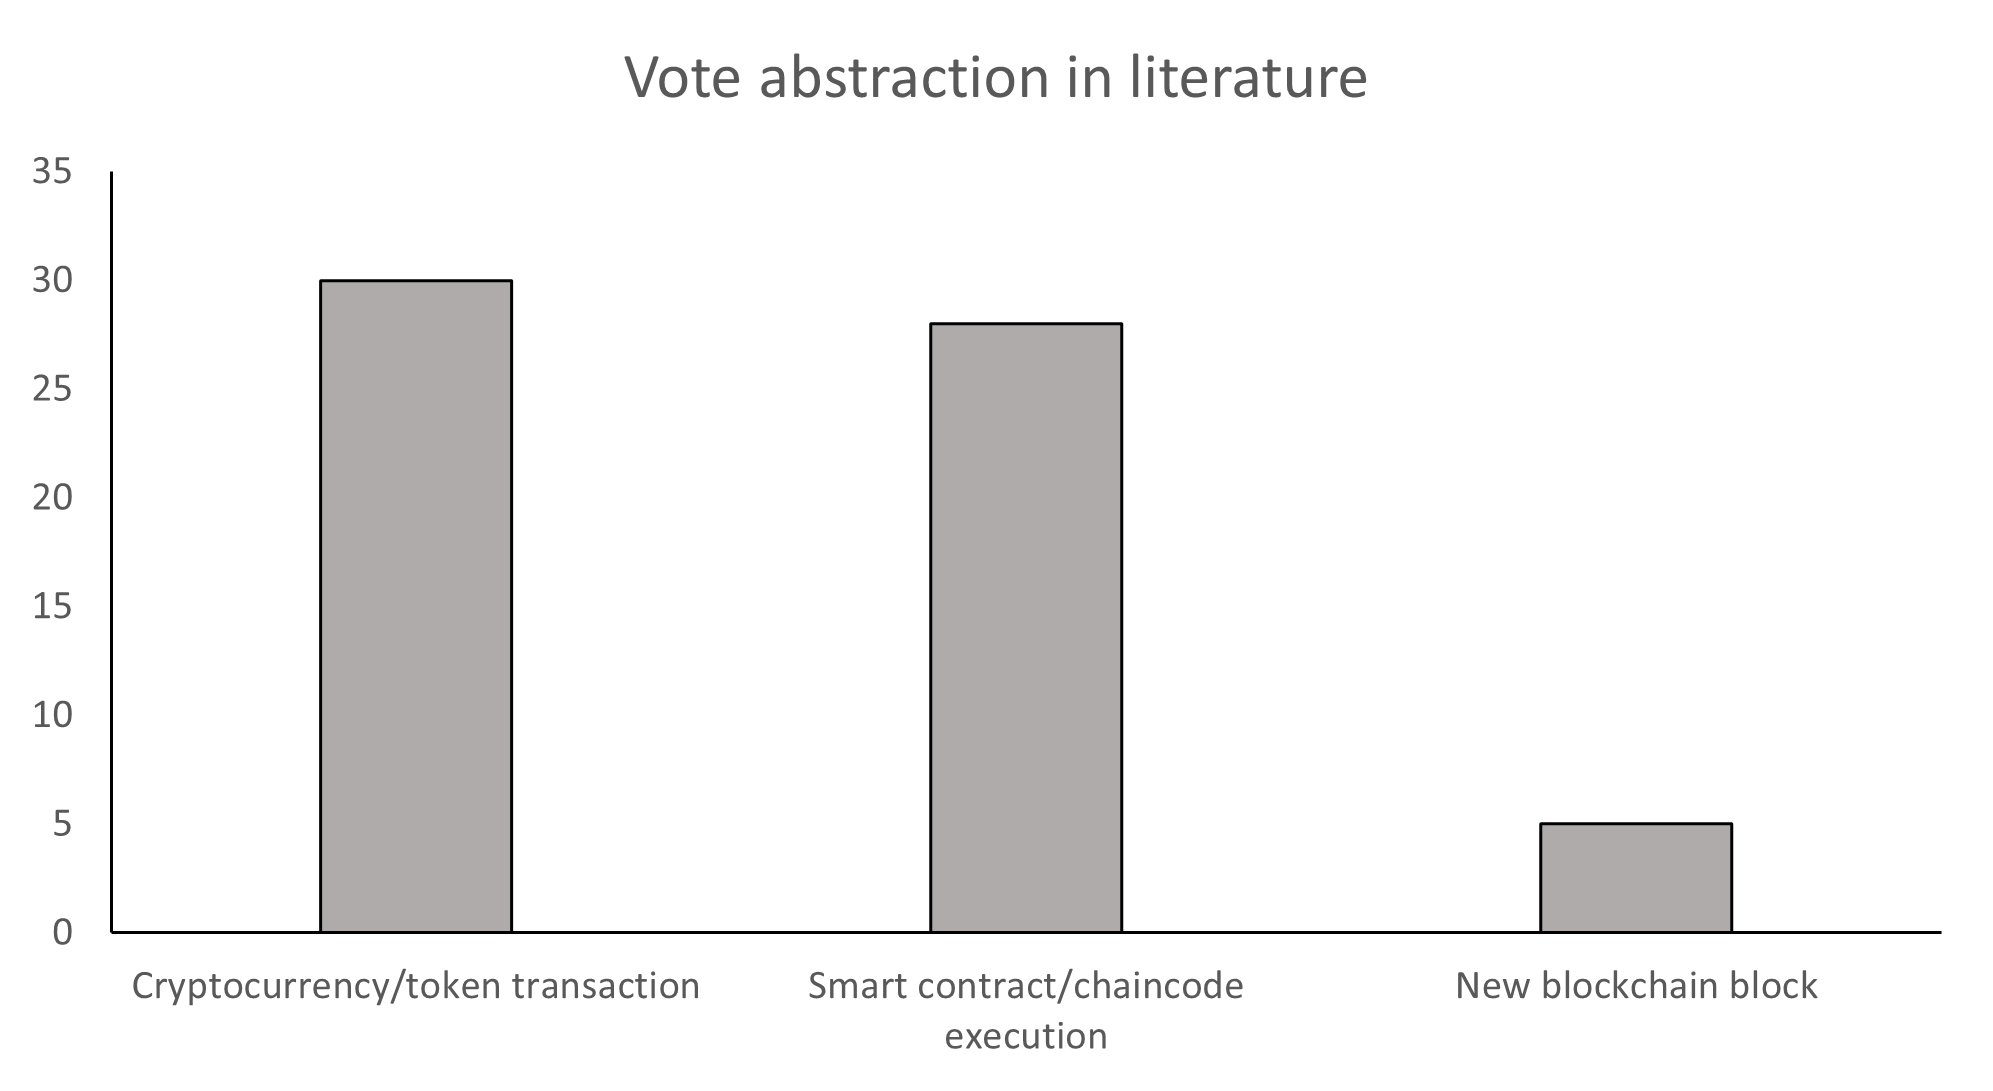
\includegraphics[width=\columnwidth]{Images/almei6.png}
    \caption{Vote abstraction methods encountered in literature.}
    \label{fig:vote-abstraction-methods}
\end{figure}

The decentralised paradigm reveals greater proximity to the academic proposals reviewed than the centralised one. Similarly, most of the real-world implementations revealed enough technical details to warrant a significant comparison to the academic papers, as well as a characterization under the same set of criteria as these, which can be evidenced from the analysis in Section \ref{real-world-decentralized-solutions}. A shorter gap between academic research and practical societal applications, along with an openness to the underlying technology, justifies this encouraging trend.
\twocolumn
\end{document}